

% 
% \mbox{}
% \thispagestyle{empty}
% \newpage

\setcounter{chapter}{2}
\chapter{Frações na reta numérica }
\setcounter{subsection}{0}
\section{EXPLORANDO O ASSUNTO }

\begin{atividade}{}

Os quadrinhos a seguir mostram uma caixa-d'água sendo enchida.
Para saber que fração da capacidade da caixa-d'água já está com água, será usada uma faixa graduada para indicar o nível de água na caixa.

\begin{table}[H]
\centering
\setlength\tabulinesep{10pt}
\begin{tabu} to \textwidth{|c|c|}
\hline

\begin{tikzpicture}[scale=2.5, x=1cm, y=1cm]



\draw [fill=brown] (-.3,0,0) -- (1.3,0,0) -- (1.3,0,1) -- (-.3,0,1) -- cycle;
\draw [fill=brown!70!black] (1.3,0,-0) -- (1.3,-.05,0) -- (1.3,-.05,1) -- (1.3,0,1);
\draw [fill=brown!70!black] (1.3,0,1) -- (1.3,-.05,1) -- (-.3,-.05,1) -- (-.3,0,1);



\draw (0,0,0) -- (1,0,0) -- (1,0,1) -- (0,0,1) -- cycle;

\draw (0,0,0) -- (0,1,0);
\draw [fill=white, opacity=.7] (0,1,0) -- (1,1,0) -- (1,1,1) -- (0,1,1) -- cycle;
\draw [fill=white, opacity=.7] (0,0,1) -- (1,0,1) -- (1,1,1) -- (0,1,1) -- cycle;

\fill [common!80] (0,.25,0) -- (1,.25,0) -- (1,.25,1) -- (0,.25,1) -- cycle;
\fill [common] (0,0,1) -- (1,0,1) -- (1,.25,1) -- (0,.25,1) -- cycle;
\fill [common] (1,0,0) -- (1,0,1) -- (1,.25,1) -- (1,.25,0) -- cycle;

\draw (1,0,1) -- (1,1,1);
\draw (1,0,0) -- (1,1,0);
\draw (0,0,1) -- (0,1,1);
\draw (1,0,0) -- (1,0,1) -- (0,0,1);

\node at (0.5,-.5,.5) {Momento 1};
\end{tikzpicture}

& 

\begin{tikzpicture}[scale=2.5, x=1cm, y=1cm]

\draw [fill=brown] (-.3,0,0) -- (1.3,0,0) -- (1.3,0,1) -- (-.3,0,1) -- cycle;
\draw [fill=brown!70!black] (1.3,0,-0) -- (1.3,-.05,0) -- (1.3,-.05,1) -- (1.3,0,1);
\draw [fill=brown!70!black] (1.3,0,1) -- (1.3,-.05,1) -- (-.3,-.05,1) -- (-.3,0,1);



\draw (0,0,0) -- (1,0,0) -- (1,0,1) -- (0,0,1) -- cycle;

\draw (0,0,0) -- (0,1,0);
\draw [fill=white, opacity=.7] (0,1,0) -- (1,1,0) -- (1,1,1) -- (0,1,1) -- cycle;
\draw [fill=white, opacity=.7] (0,0,1) -- (1,0,1) -- (1,1,1) -- (0,1,1) -- cycle;

\fill [common!80] (0,.5,0) -- (1,.5,0) -- (1,.5,1) -- (0,.5,1) -- cycle;
\fill [common] (0,0,1) -- (1,0,1) -- (1,.5,1) -- (0,.5,1) -- cycle;
\fill [common] (1,0,0) -- (1,0,1) -- (1,.5,1) -- (1,.5,0) -- cycle;

\draw (1,0,1) -- (1,1,1);
\draw (1,0,0) -- (1,1,0);
\draw (0,0,1) -- (0,1,1);
\draw (1,0,0) -- (1,0,1) -- (0,0,1);
\draw (0,1,0) -- (1,1,0) -- (1,1,1) -- (0,1,1) -- cycle;

\node at (0.5,-.5,.5) {Momento 2};
\end{tikzpicture} \\

\hline

\begin{tikzpicture}[scale=2.5, x=1cm, y=1cm]

\draw [fill=brown] (-.3,0,0) -- (1.3,0,0) -- (1.3,0,1) -- (-.3,0,1) -- cycle;
\draw [fill=brown!70!black] (1.3,0,-0) -- (1.3,-.05,0) -- (1.3,-.05,1) -- (1.3,0,1);
\draw [fill=brown!70!black] (1.3,0,1) -- (1.3,-.05,1) -- (-.3,-.05,1) -- (-.3,0,1);



\draw (0,0,0) -- (1,0,0) -- (1,0,1) -- (0,0,1) -- cycle;

\draw (0,0,0) -- (0,1,0);
\draw [fill=white, opacity=.7] (0,1,0) -- (1,1,0) -- (1,1,1) -- (0,1,1) -- cycle;
\draw [fill=white, opacity=.7] (0,0,1) -- (1,0,1) -- (1,1,1) -- (0,1,1) -- cycle;

\fill [common!80] (0,.75,0) -- (1,.75,0) -- (1,.75,1) -- (0,.75,1) -- cycle;
\fill [common] (0,0,1) -- (1,0,1) -- (1,.75,1) -- (0,.75,1) -- cycle;
\fill [common] (1,0,0) -- (1,0,1) -- (1,.75,1) -- (1,.75,0) -- cycle;

\draw (1,0,1) -- (1,1,1);
\draw (1,0,0) -- (1,1,0);
\draw (0,0,1) -- (0,1,1);
\draw (1,0,0) -- (1,0,1) -- (0,0,1);
\draw (0,1,0) -- (1,1,0) -- (1,1,1) -- (0,1,1) -- cycle;

\node at (0.5,-.5,.5) {Momento 3};
\end{tikzpicture}

& 
\begin{tikzpicture}[scale=2.5, x=1cm, y=1cm]

\draw [fill=brown] (-.3,0,0) -- (1.3,0,0) -- (1.3,0,1) -- (-.3,0,1) -- cycle;
\draw [fill=brown!70!black] (1.3,0,-0) -- (1.3,-.05,0) -- (1.3,-.05,1) -- (1.3,0,1);
\draw [fill=brown!70!black] (1.3,0,1) -- (1.3,-.05,1) -- (-.3,-.05,1) -- (-.3,0,1);



\draw (0,0,0) -- (1,0,0) -- (1,0,1) -- (0,0,1) -- cycle;

\draw (0,0,0) -- (0,1,0);
\draw [fill=white, opacity=.7] (0,1,0) -- (1,1,0) -- (1,1,1) -- (0,1,1) -- cycle;
\draw [fill=white, opacity=.7] (0,0,1) -- (1,0,1) -- (1,1,1) -- (0,1,1) -- cycle;


\fill [common!80] (0,1,0) -- (1,1,0) -- (1,1,1) -- (0,1,1) -- cycle;
\fill [common] (0,0,1) -- (1,0,1) -- (1,1,1) -- (0,1,1) -- cycle;
\fill [common] (1,0,0) -- (1,0,1) -- (1,1,1) -- (1,1,0) -- cycle;

\draw (1,0,1) -- (1,1,1);
\draw (1,0,0) -- (1,1,0);
\draw (0,0,1) -- (0,1,1);
\draw (1,0,0) -- (1,0,1) -- (0,0,1);
\draw (0,1,0) -- (1,1,0) -- (1,1,1) -- (0,1,1) -- cycle;


\node at (0.5,-.5,.5) {Momento 4};
\end{tikzpicture} \\
\hline
\end{tabu}
\end{table}

Escolha, para cada um dos momentos, a graduação que lhe parece mais adequada para registrar a quantidade de água representada em cada uma das imagens. Explique sua escolha.

\begin{enumerate}
\begin{multicols}{2}

\item\adjustbox{valign=t}{
\begin{tikzpicture}[scale=2.5, x=1cm, y=1cm]

\draw [fill=brown] (-.3,0,0) -- (1.3,0,0) -- (1.3,0,1) -- (-.3,0,1) -- cycle;
\draw [fill=brown!70!black] (1.3,0,-0) -- (1.3,-.05,0) -- (1.3,-.05,1) -- (1.3,0,1);
\draw [fill=brown!70!black] (1.3,0,1) -- (1.3,-.05,1) -- (-.3,-.05,1) -- (-.3,0,1);

\draw [fill=white, opacity=.7] (0,0,0) -- (1,0,0) -- (1,0,1) -- (0,0,1) -- cycle;
\draw [fill=white, opacity=.7] (0,0,0) -- (0,1,0) -- (1,1,0) -- (1,0,0) -- cycle;
\draw [fill=white, opacity=.7] (0,0,0) -- (0,1,0) -- (0,1,1) -- (0,0,1) -- cycle;
\draw [fill=white, opacity=.7] (0,0,1) -- (1,0,1) -- (1,1,1) -- (0,1,1) -- cycle;
\draw [fill=white, opacity=.7] (1,0,0) -- (1,0,1) -- (1,1,1) -- (1,1,0) -- cycle;
\draw [fill=white, opacity=.7] (0,1,0) -- (1,1,0) -- (1,1,1) -- (0,1,1) -- cycle;

\filldraw [fill=white] (0,-.05,1) rectangle (0.3,1.05,1);
\draw [|-|] (.1,0,1) -- (.1,1,1) node [right, scale=.75, xshift=.05cm] {\footnotesize 1} node [ right, pos=0, scale=.75, xshift=.05cm]{\footnotesize 0};
\draw [|-|] (.1,0,1) -- (.1,.5,1) node [right, scale=.75, xshift=.025cm,pos=.5] {\footnotesize $\frac{1}{2}$};

\end{tikzpicture}  
}
\item\adjustbox{valign=t}{
\begin{tikzpicture}[scale=2.5, x=1cm, y=1cm]

\draw [fill=brown] (-.3,0,0) -- (1.3,0,0) -- (1.3,0,1) -- (-.3,0,1) -- cycle;
\draw [fill=brown!70!black] (1.3,0,-0) -- (1.3,-.05,0) -- (1.3,-.05,1) -- (1.3,0,1);
\draw [fill=brown!70!black] (1.3,0,1) -- (1.3,-.05,1) -- (-.3,-.05,1) -- (-.3,0,1);



\draw [fill=white, opacity=.7] (0,0,0) -- (1,0,0) -- (1,0,1) -- (0,0,1) -- cycle;
\draw [fill=white, opacity=.7] (0,0,0) -- (0,1,0) -- (1,1,0) -- (1,0,0) -- cycle;
\draw [fill=white, opacity=.7] (0,0,0) -- (0,1,0) -- (0,1,1) -- (0,0,1) -- cycle;
\draw [fill=white, opacity=.7] (0,0,1) -- (1,0,1) -- (1,1,1) -- (0,1,1) -- cycle;
\draw [fill=white, opacity=.7] (1,0,0) -- (1,0,1) -- (1,1,1) -- (1,1,0) -- cycle;
\draw [fill=white, opacity=.7] (0,1,0) -- (1,1,0) -- (1,1,1) -- (0,1,1) -- cycle;

\filldraw [fill=white] (0,-.05,1) rectangle (0.3,1.05,1);
\draw [|-|] (.1,0,1) -- (.1,1,1) node [right, scale=.75, xshift=.05cm] {\footnotesize 1} node [ right, pos=0, scale=.75, xshift=.05cm]{\footnotesize 0};
\draw [|-|] (.1,0,1) -- (.1,.5,1) node [right, scale=.75, xshift=.025cm] {\footnotesize $\frac{1}{2}$};
\draw [|-|] (.1,0,1) -- (.1,.25,1) node [right, scale=.75, xshift=.025cm] {\footnotesize $\frac{1}{4}$};
\draw [|-|] (.1,0,1) -- (.1,.75,1) node [right, scale=.75, xshift=.025cm] { \footnotesize $\frac{3}{4}$};


\end{tikzpicture}  
}
\end{multicols}

\begin{multicols}{2}
\item\adjustbox{valign=t}{
\begin{tikzpicture}[scale=2.5, x=1cm, y=1cm]

\draw [fill=brown] (-.3,0,0) -- (1.3,0,0) -- (1.3,0,1) -- (-.3,0,1) -- cycle;
\draw [fill=brown!70!black] (1.3,0,-0) -- (1.3,-.05,0) -- (1.3,-.05,1) -- (1.3,0,1);
\draw [fill=brown!70!black] (1.3,0,1) -- (1.3,-.05,1) -- (-.3,-.05,1) -- (-.3,0,1);



\draw [fill=white, opacity=.7] (0,0,0) -- (1,0,0) -- (1,0,1) -- (0,0,1) -- cycle;
\draw [fill=white, opacity=.7] (0,0,0) -- (0,1,0) -- (1,1,0) -- (1,0,0) -- cycle;
\draw [fill=white, opacity=.7] (0,0,0) -- (0,1,0) -- (0,1,1) -- (0,0,1) -- cycle;
\draw [fill=white, opacity=.7] (0,0,1) -- (1,0,1) -- (1,1,1) -- (0,1,1) -- cycle;
\draw [fill=white, opacity=.7] (1,0,0) -- (1,0,1) -- (1,1,1) -- (1,1,0) -- cycle;
\draw [fill=white, opacity=.7] (0,1,0) -- (1,1,0) -- (1,1,1) -- (0,1,1) -- cycle;

\filldraw [fill=white] (0,-.05,1) rectangle (0.3,1.05,1);
\draw [|-|] (.1,0,1) -- (.1,1,1) node [right, scale=.75, xshift=.05cm] {\footnotesize 1} node [ right, pos=0, scale=.75, xshift=.05cm]{\footnotesize 0};

\draw [|-|] (.1,0,1) -- (.1,.75,1) node [right, scale=.75, xshift=.025cm] { \footnotesize $\frac{1}{2}$};  
\end{tikzpicture}
}


\item\adjustbox{valign=t}{
\begin{tikzpicture}[scale=2.5, x=1cm, y=1cm]

\draw [fill=brown] (-.3,0,0) -- (1.3,0,0) -- (1.3,0,1) -- (-.3,0,1) -- cycle;
\draw [fill=brown!70!black] (1.3,0,-0) -- (1.3,-.05,0) -- (1.3,-.05,1) -- (1.3,0,1);
\draw [fill=brown!70!black] (1.3,0,1) -- (1.3,-.05,1) -- (-.3,-.05,1) -- (-.3,0,1);



\draw [fill=white, opacity=.7] (0,0,0) -- (1,0,0) -- (1,0,1) -- (0,0,1) -- cycle;
\draw [fill=white, opacity=.7] (0,0,0) -- (0,1,0) -- (1,1,0) -- (1,0,0) -- cycle;
\draw [fill=white, opacity=.7] (0,0,0) -- (0,1,0) -- (0,1,1) -- (0,0,1) -- cycle;
\draw [fill=white, opacity=.7] (0,0,1) -- (1,0,1) -- (1,1,1) -- (0,1,1) -- cycle;
\draw [fill=white, opacity=.7] (1,0,0) -- (1,0,1) -- (1,1,1) -- (1,1,0) -- cycle;
\draw [fill=white, opacity=.7] (0,1,0) -- (1,1,0) -- (1,1,1) -- (0,1,1) -- cycle;

\filldraw [fill=white] (0,-.05,1) rectangle (0.3,1.05,1);
\draw [|-|] (.1,0,1) -- (.1,1,1) node [right, scale=.75, xshift=.05cm] {\footnotesize 1} node [ right, pos=0, scale=.75, xshift=.05cm]{\footnotesize 0};
\draw [|-|] (.1,0,1) -- (.1,.5,1) node [right, scale=.75, xshift=.025cm] {\footnotesize $\frac{1}{3}$};
\draw [|-|] (.1,0,1) -- (.1,.25,1) node [right, scale=.75, xshift=.025cm] {\footnotesize $\frac{1}{4}$};
\draw [|-|] (.1,0,1) -- (.1,.75,1) node [right, scale=.75, xshift=.025cm] { \footnotesize $\frac{1}{2}$};


\end{tikzpicture}
}
\end{multicols}

\begin{multicols}{2}

\item\adjustbox{valign=t}{
\begin{tikzpicture}[scale=2.5, x=1cm, y=1cm]

\draw [fill=brown] (-.3,0,0) -- (1.3,0,0) -- (1.3,0,1) -- (-.3,0,1) -- cycle;
\draw [fill=brown!70!black] (1.3,0,-0) -- (1.3,-.05,0) -- (1.3,-.05,1) -- (1.3,0,1);
\draw [fill=brown!70!black] (1.3,0,1) -- (1.3,-.05,1) -- (-.3,-.05,1) -- (-.3,0,1);


\draw [fill=white, opacity=.7] (0,0,0) -- (1,0,0) -- (1,0,1) -- (0,0,1) -- cycle;
\draw [fill=white, opacity=.7] (0,0,0) -- (0,1,0) -- (1,1,0) -- (1,0,0) -- cycle;
\draw [fill=white, opacity=.7] (0,0,0) -- (0,1,0) -- (0,1,1) -- (0,0,1) -- cycle;
\draw [fill=white, opacity=.7] (0,0,1) -- (1,0,1) -- (1,1,1) -- (0,1,1) -- cycle;
\draw [fill=white, opacity=.7] (1,0,0) -- (1,0,1) -- (1,1,1) -- (1,1,0) -- cycle;
\draw [fill=white, opacity=.7] (0,1,0) -- (1,1,0) -- (1,1,1) -- (0,1,1) -- cycle;

\filldraw [fill=white] (0,-.05,1) rectangle (0.3,1.05,1);
\draw [|-|] (.1,0,1) -- (.1,1,1) node [right, scale=.75, xshift=.05cm] {\footnotesize 1} node [ right, pos=0, scale=.75, xshift=.05cm]{\footnotesize 0};
\draw [|-|] (.1,0,1) -- (.1,.5,1) node [right, scale=.75, xshift=.025cm] {\footnotesize $\frac{1}{2}$};



\end{tikzpicture}


}
\end{multicols}
\end{enumerate}
 %     \begin{center}
 %     \begin{tabular}{m{.3\textwidth}m{.3\textwidth}m{.3\textwidth}}
 % \parbox[b][.3cm][t]{.3cm}{a)}  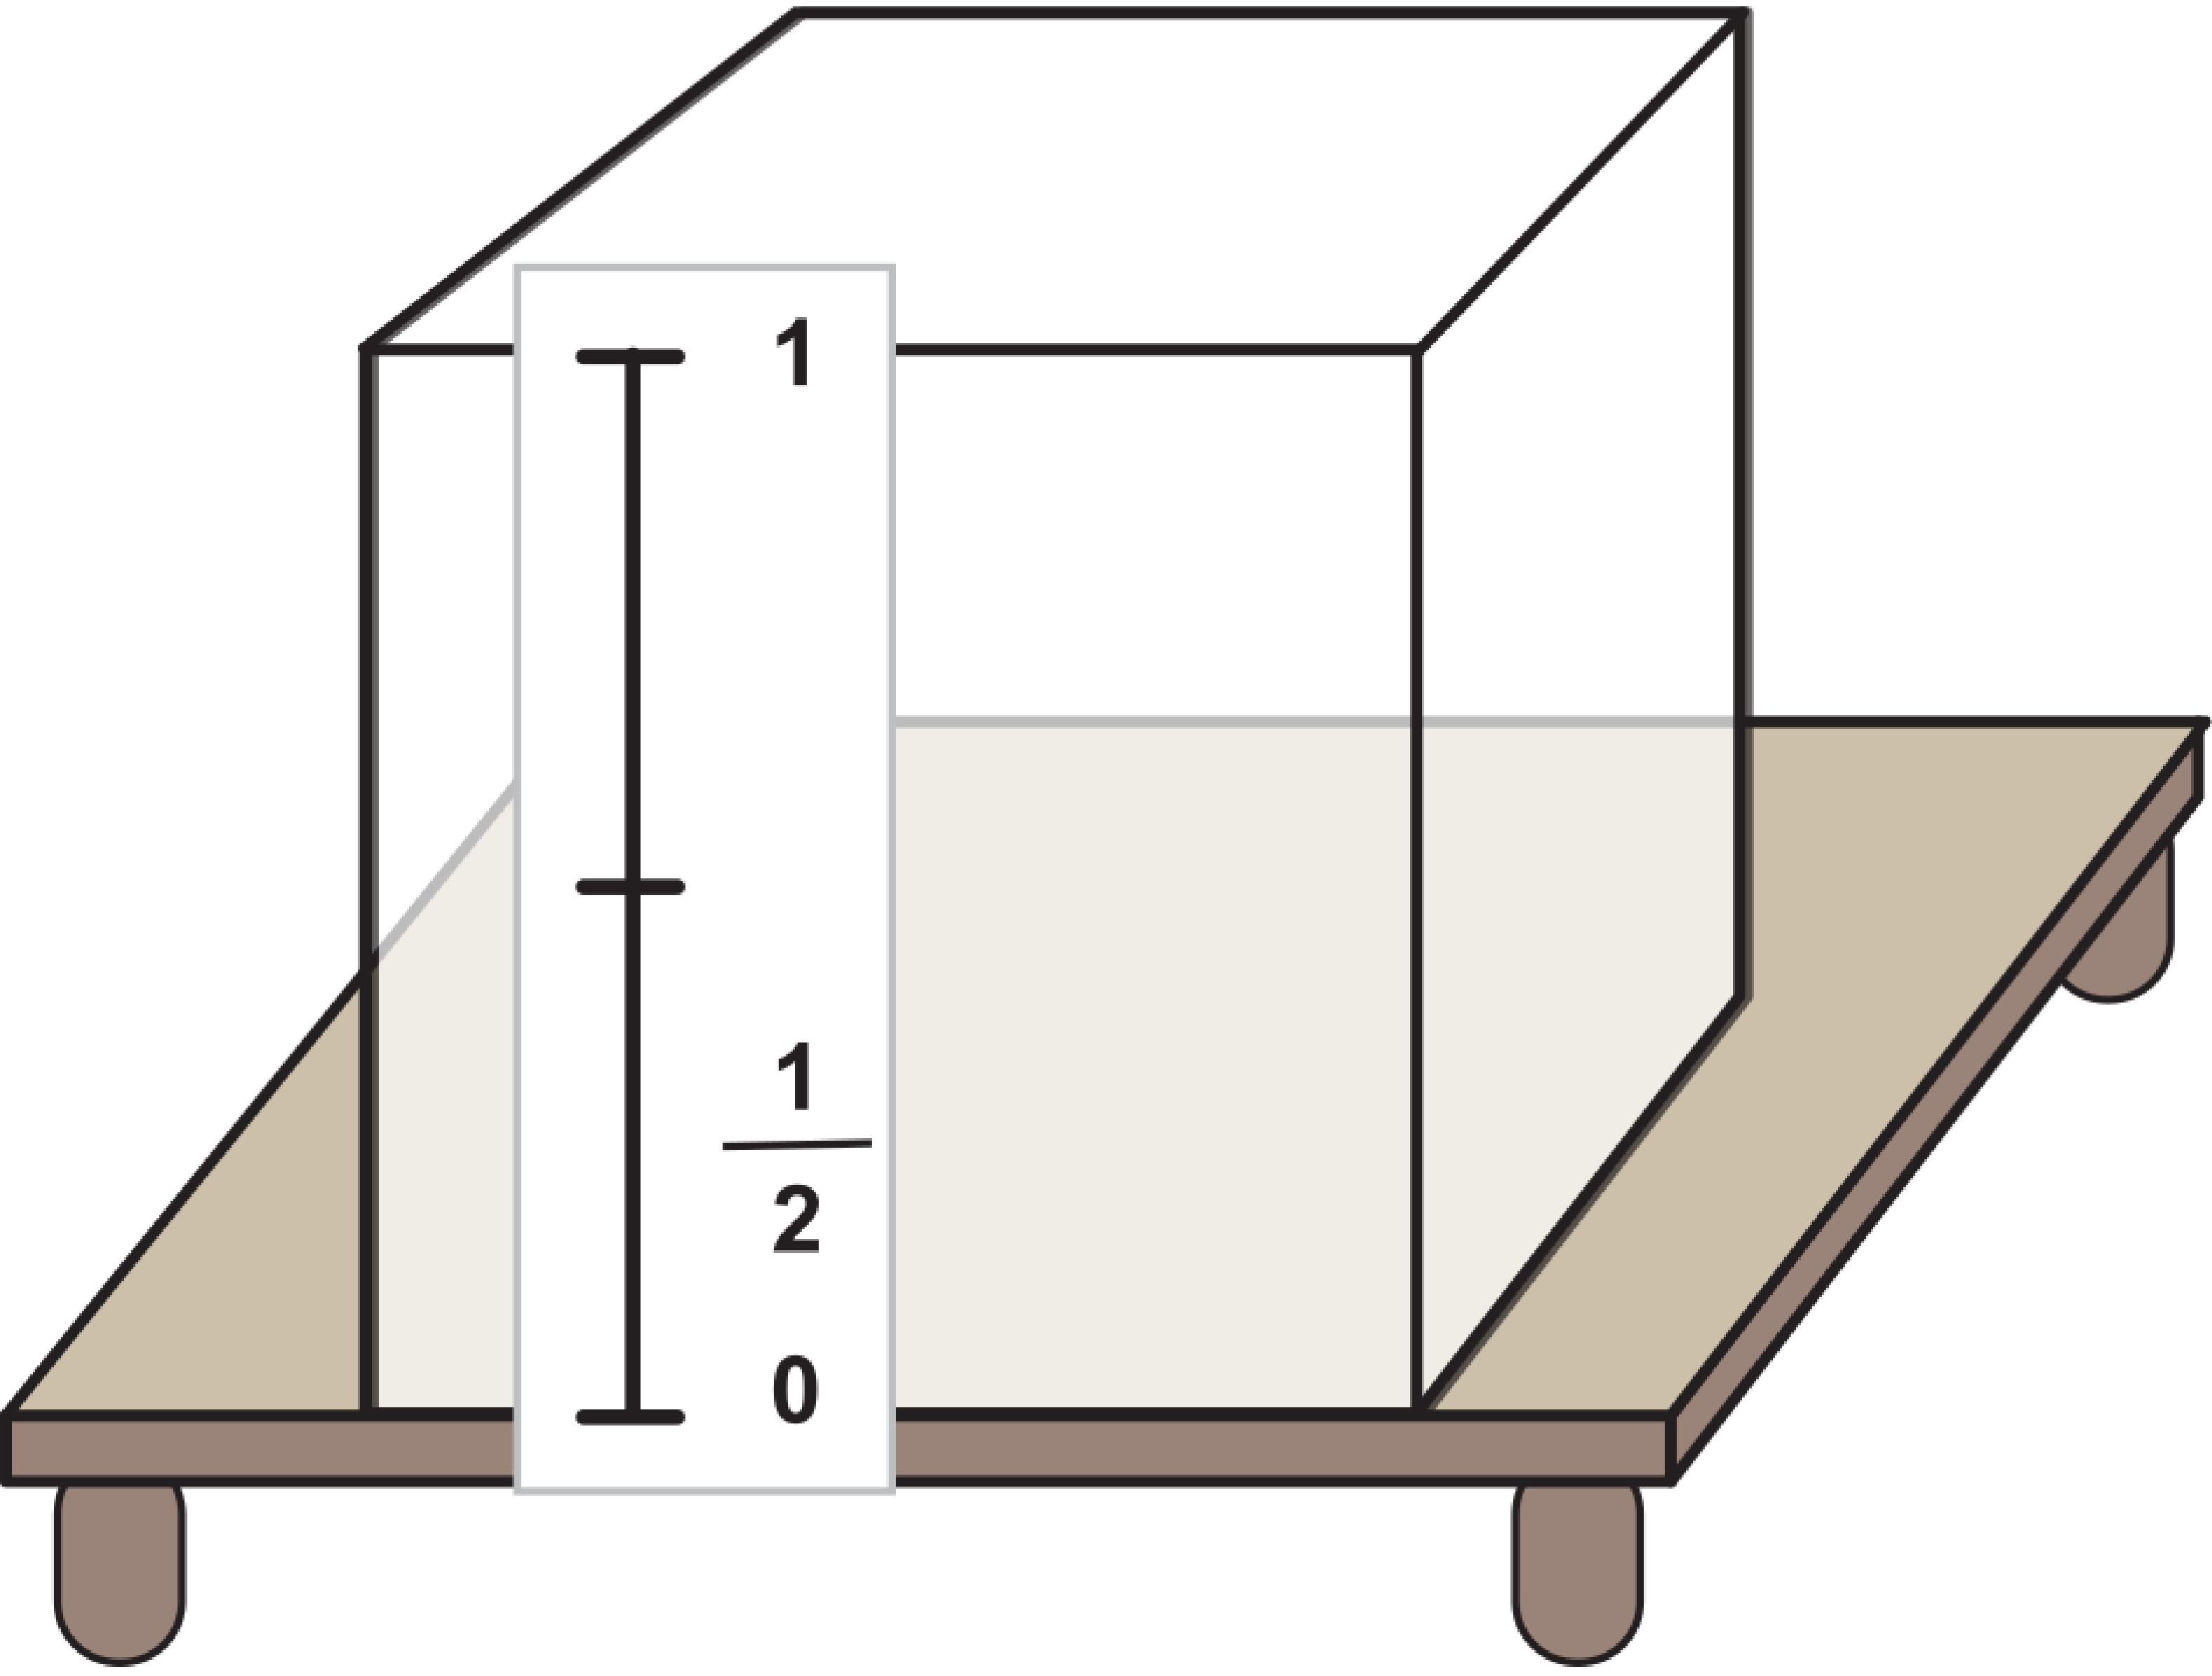
\includegraphics[width=145pt, keepaspectratio]{../figuras/licao03/ativ1_fig05.png} &
 % \parbox[b][.3cm][t]{.3cm}{b)}  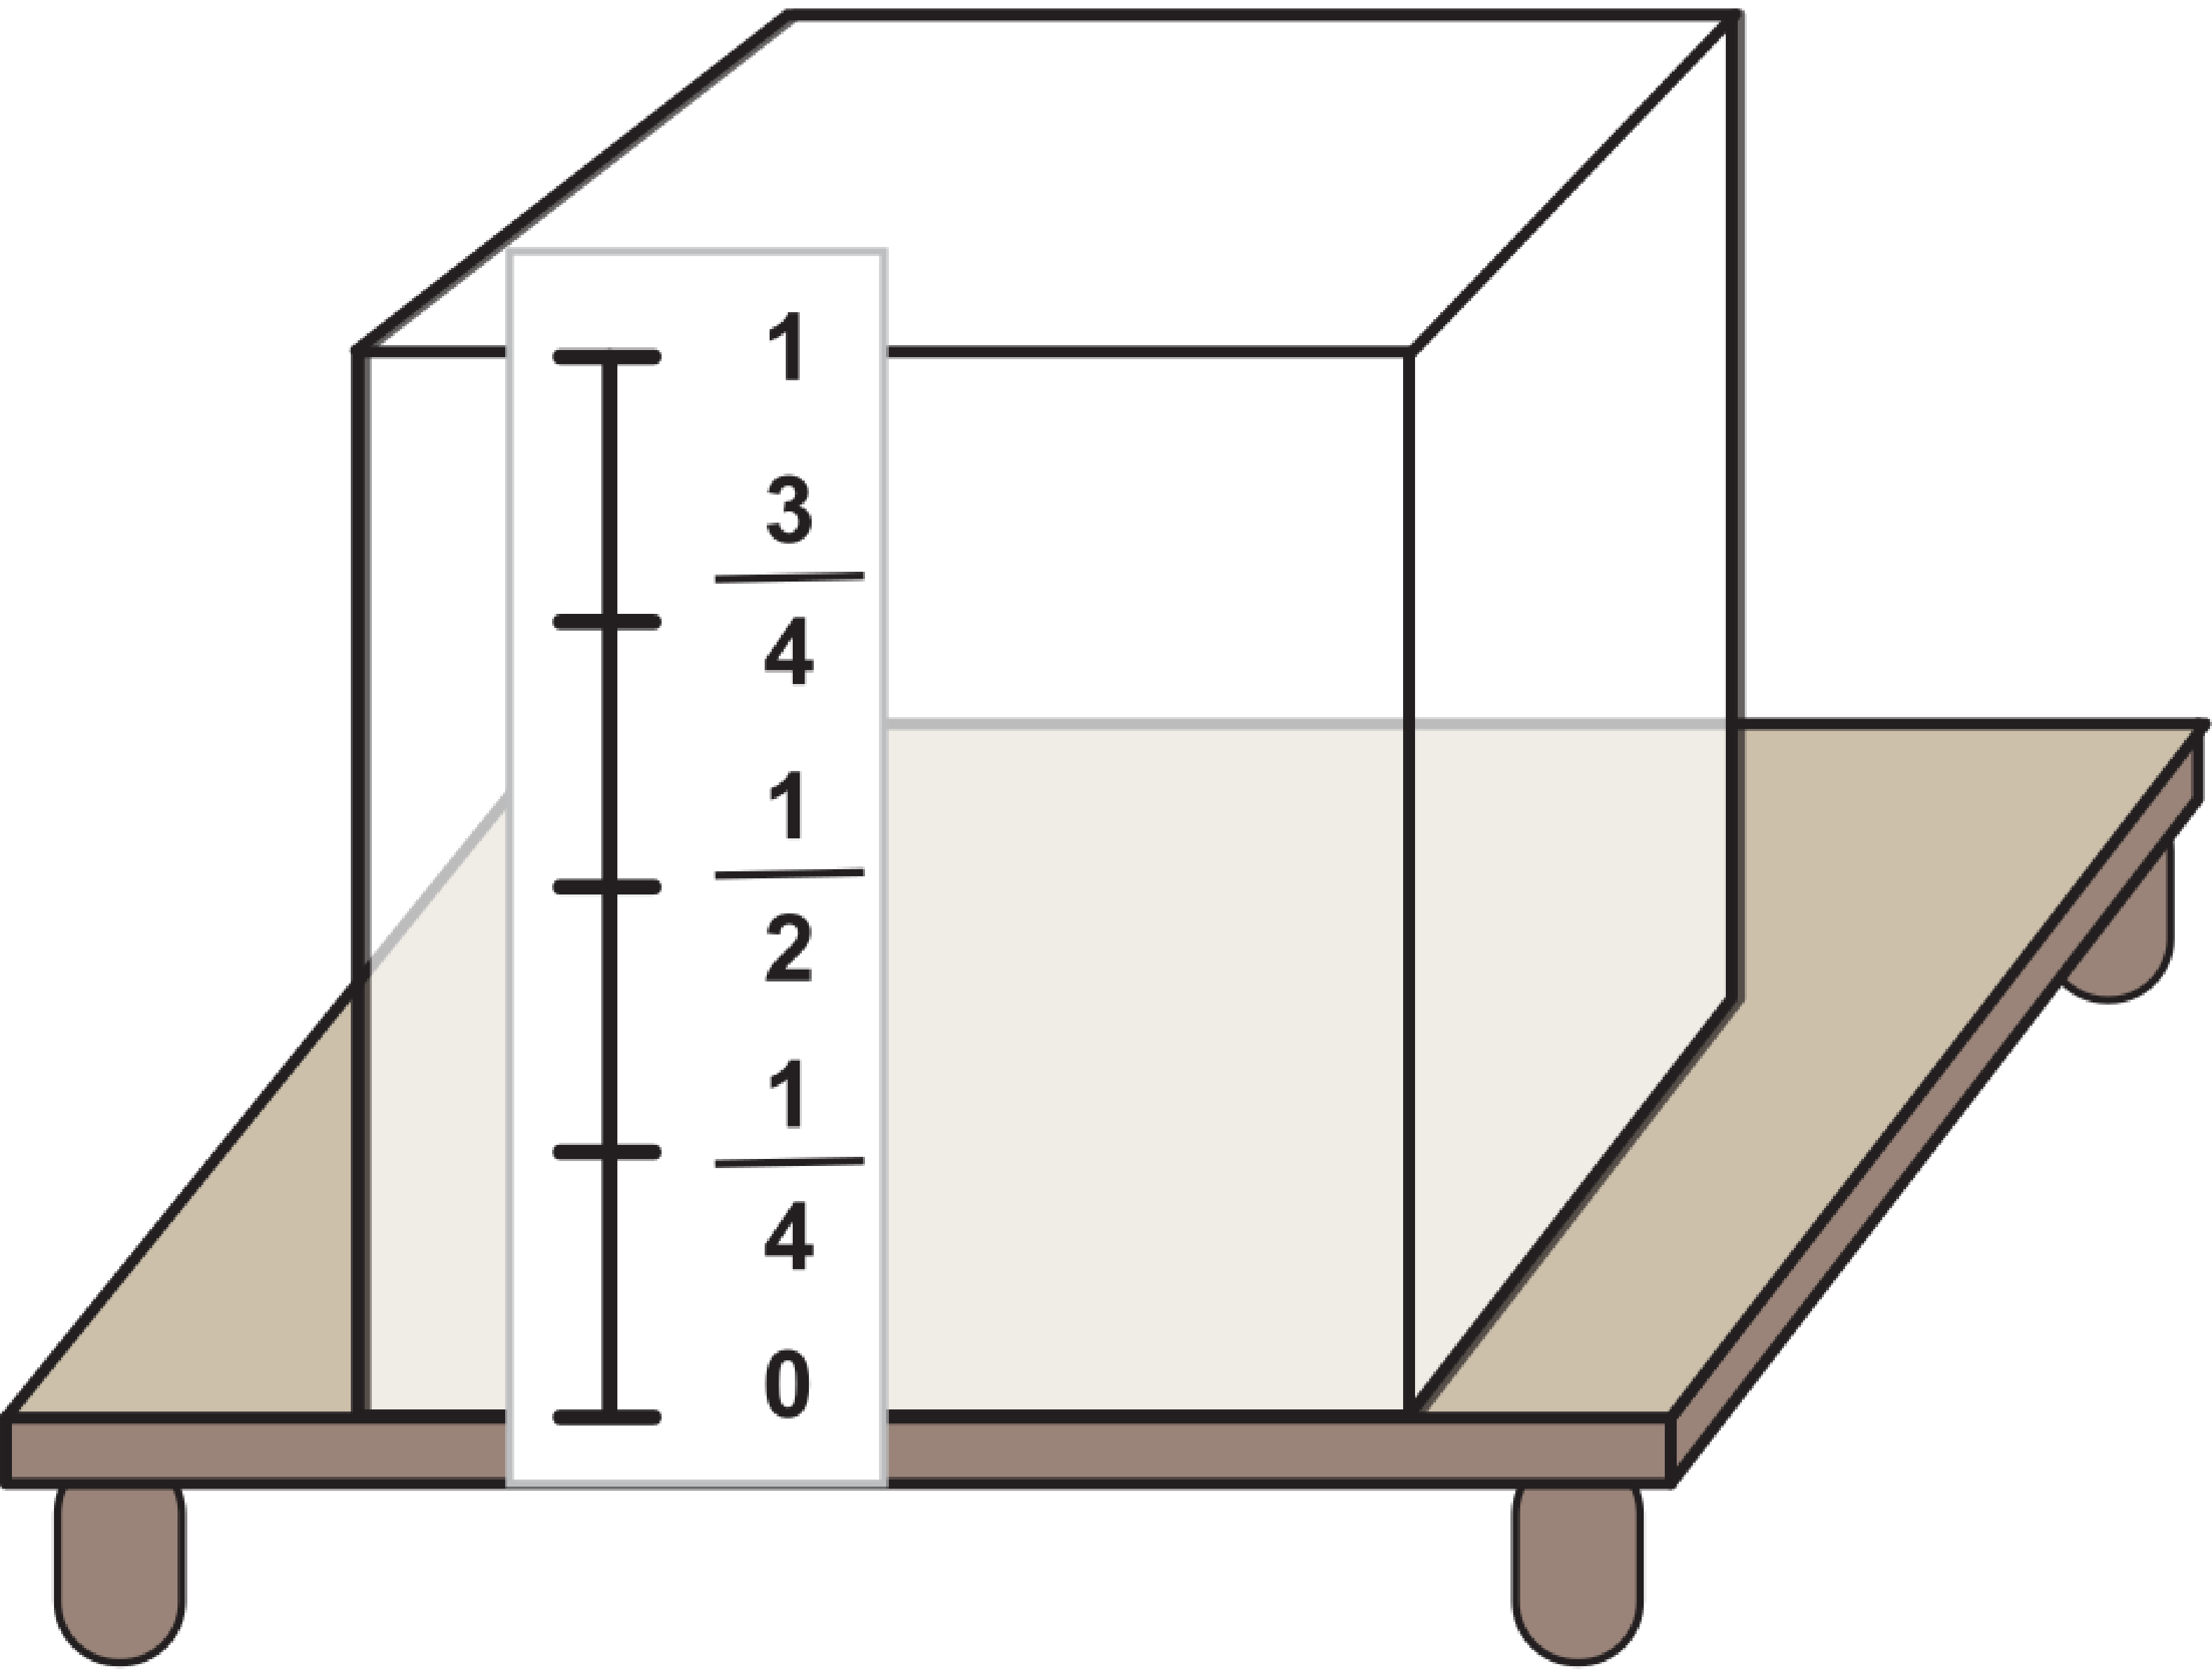
\includegraphics[width=145pt, keepaspectratio]{../figuras/licao03/ativ1_fig06.png} &
 %  \parbox[b][.3cm][t]{.3cm}{c)}  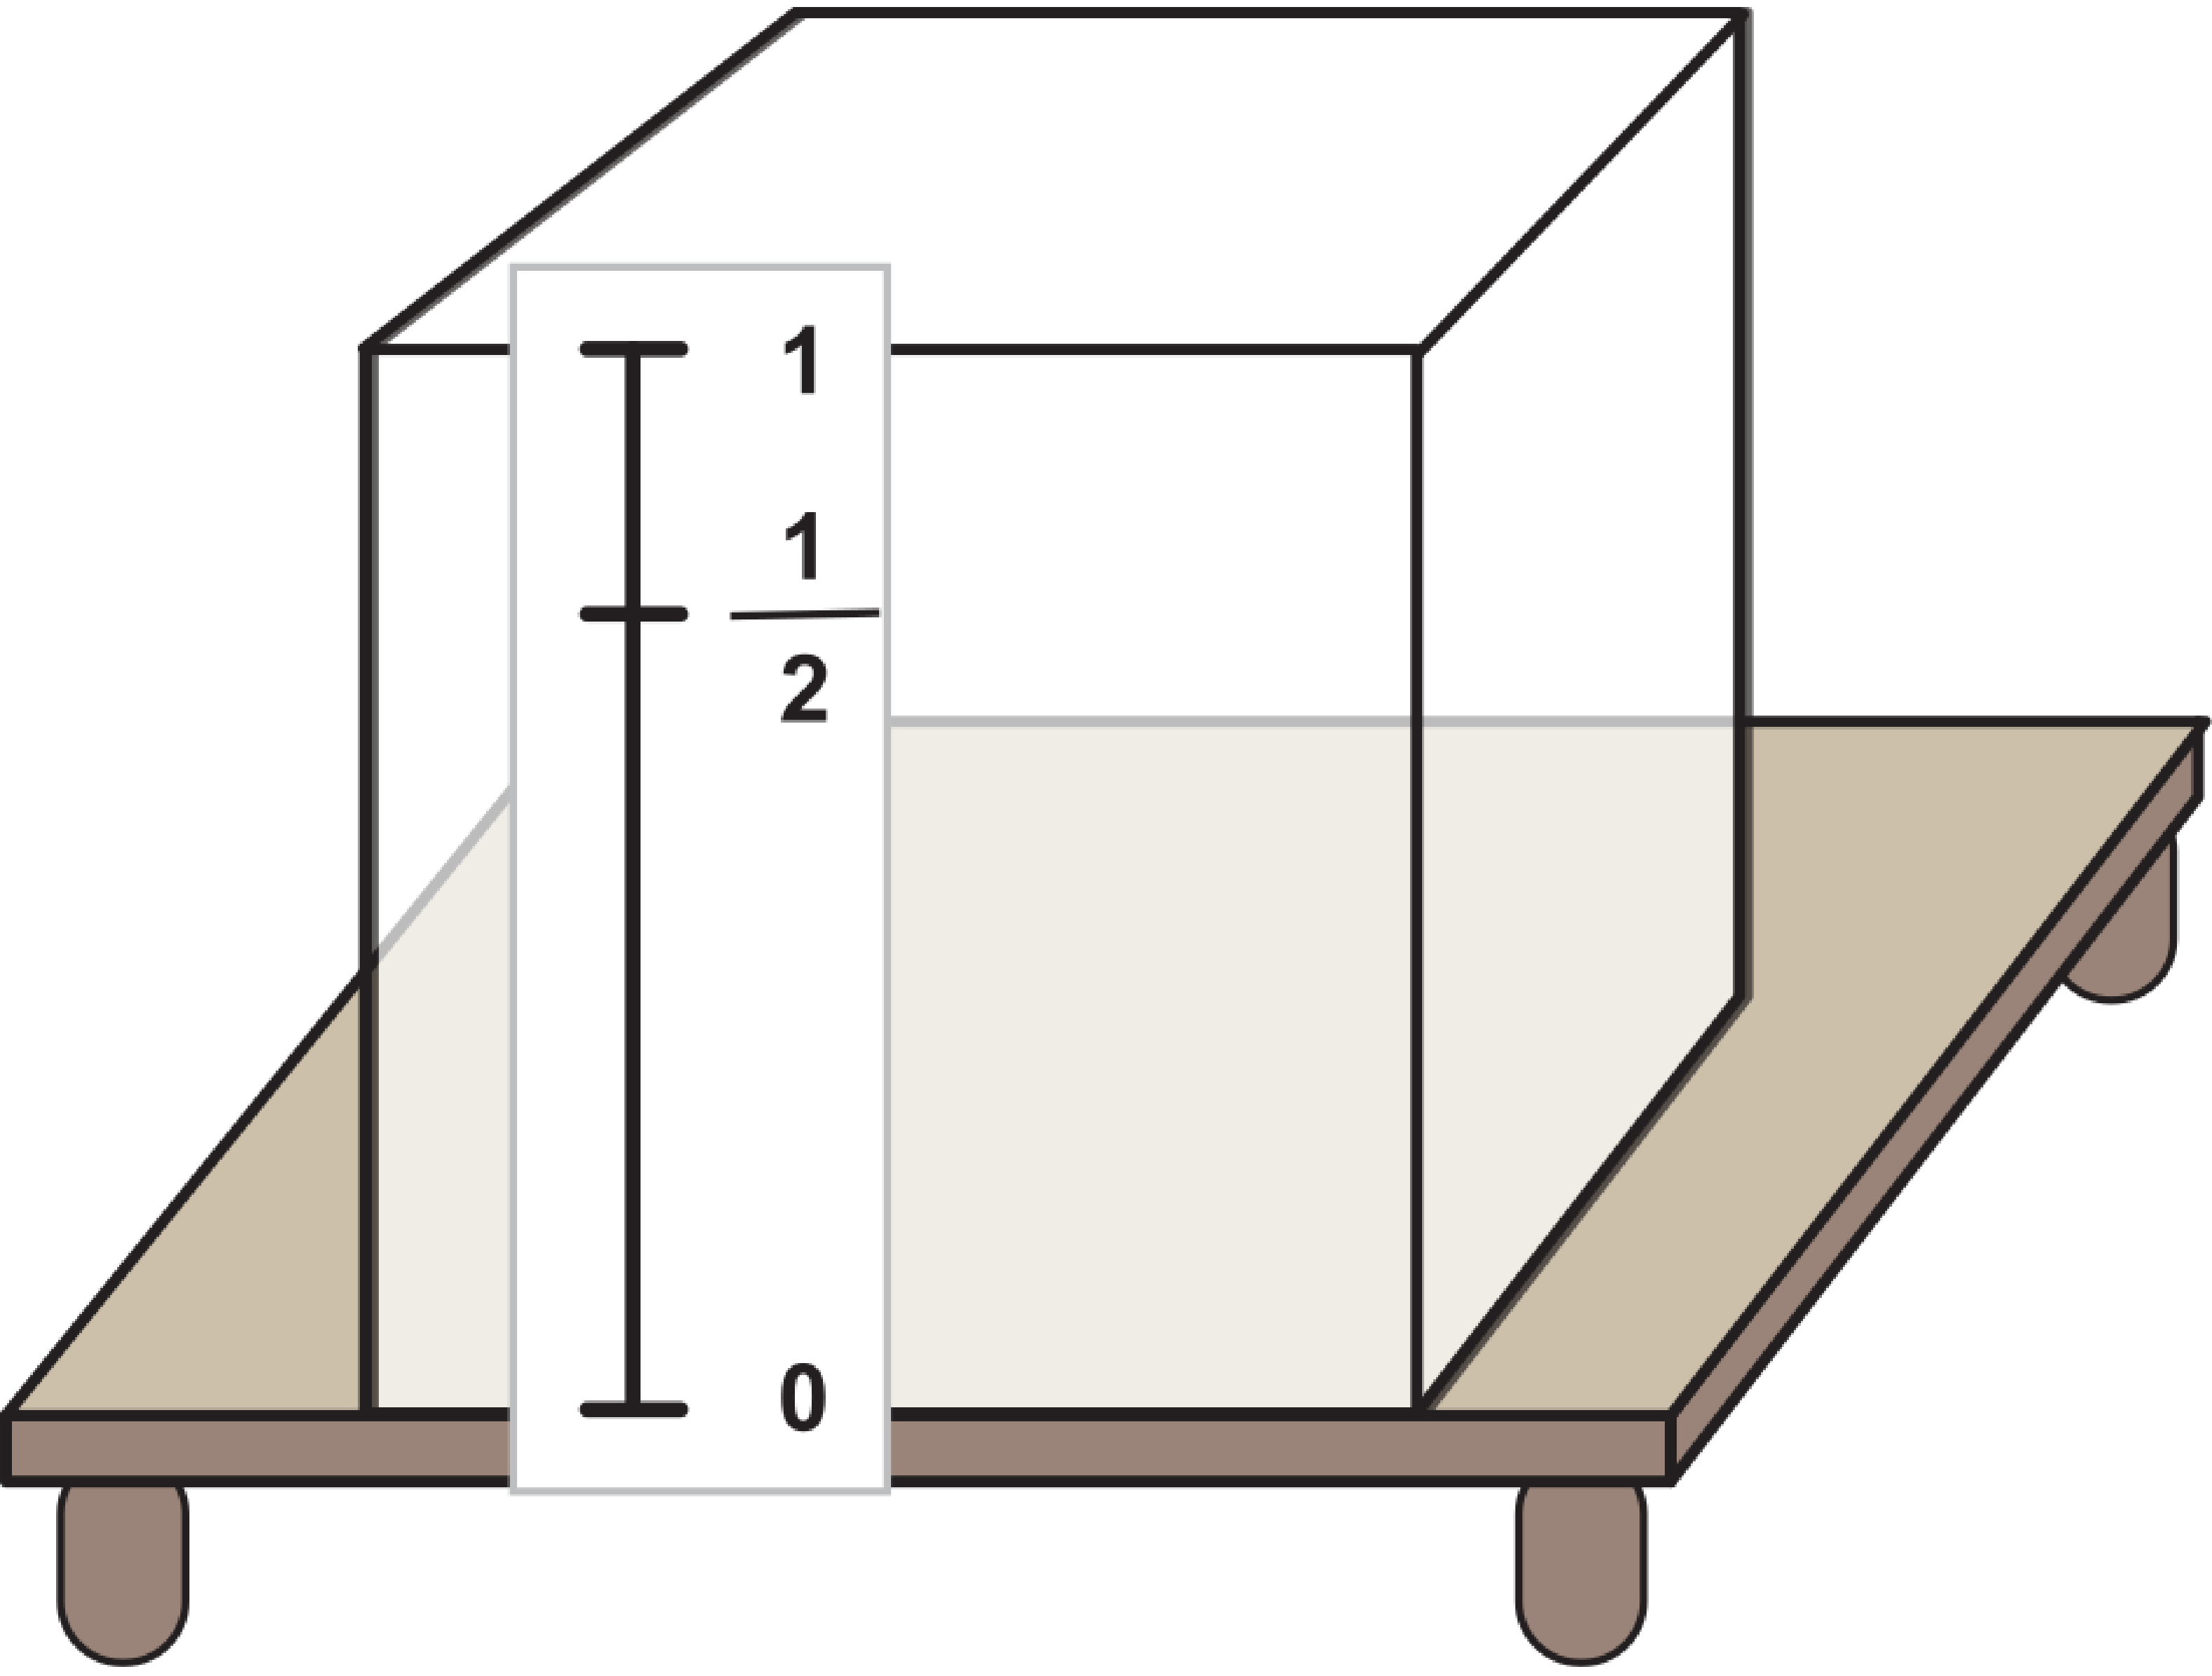
\includegraphics[width=145pt, keepaspectratio]{../figuras/licao03/ativ1_fig07.png}
 %   \end{tabular}

 %  \begin{tabular}{m{.3\textwidth}m{.3\textwidth}}
 %  \parbox[b][0.3cm][t]{.3cm}{d)}  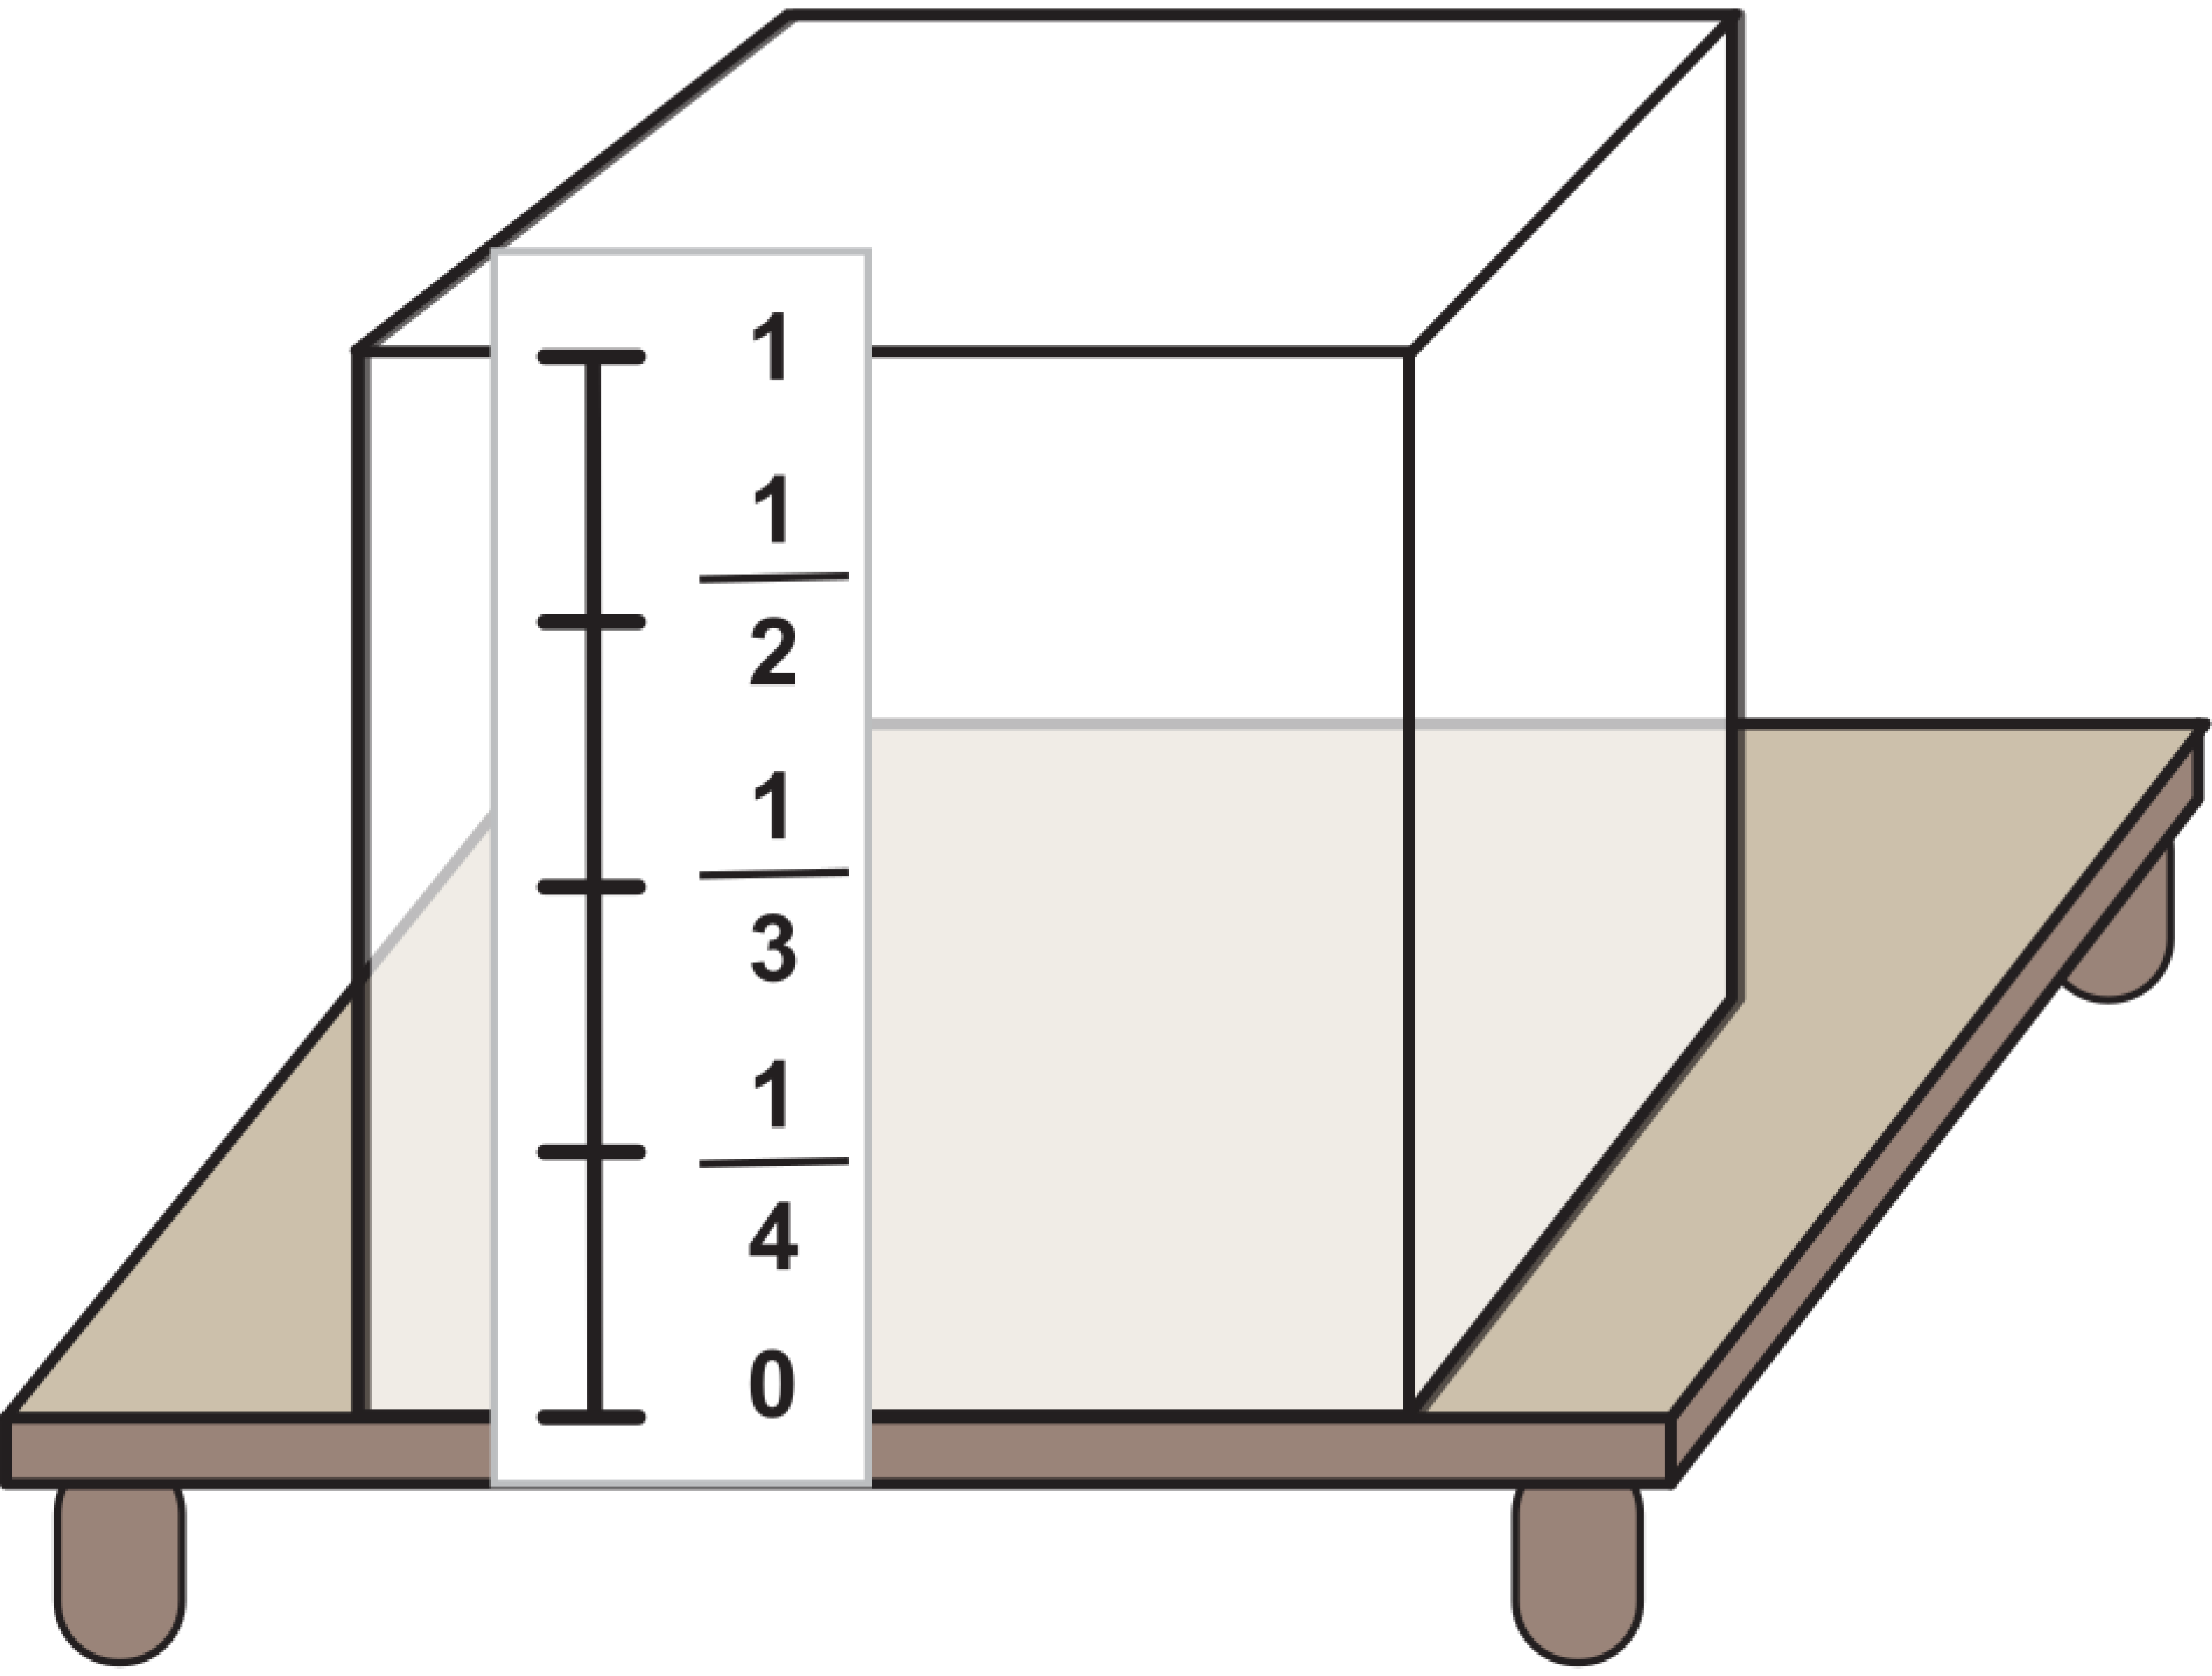
\includegraphics[width=145pt, keepaspectratio]{../figuras/licao03/ativ1_fig08.png}&
 %  \parbox[b][0.3cm][t]{.3cm}{e)}  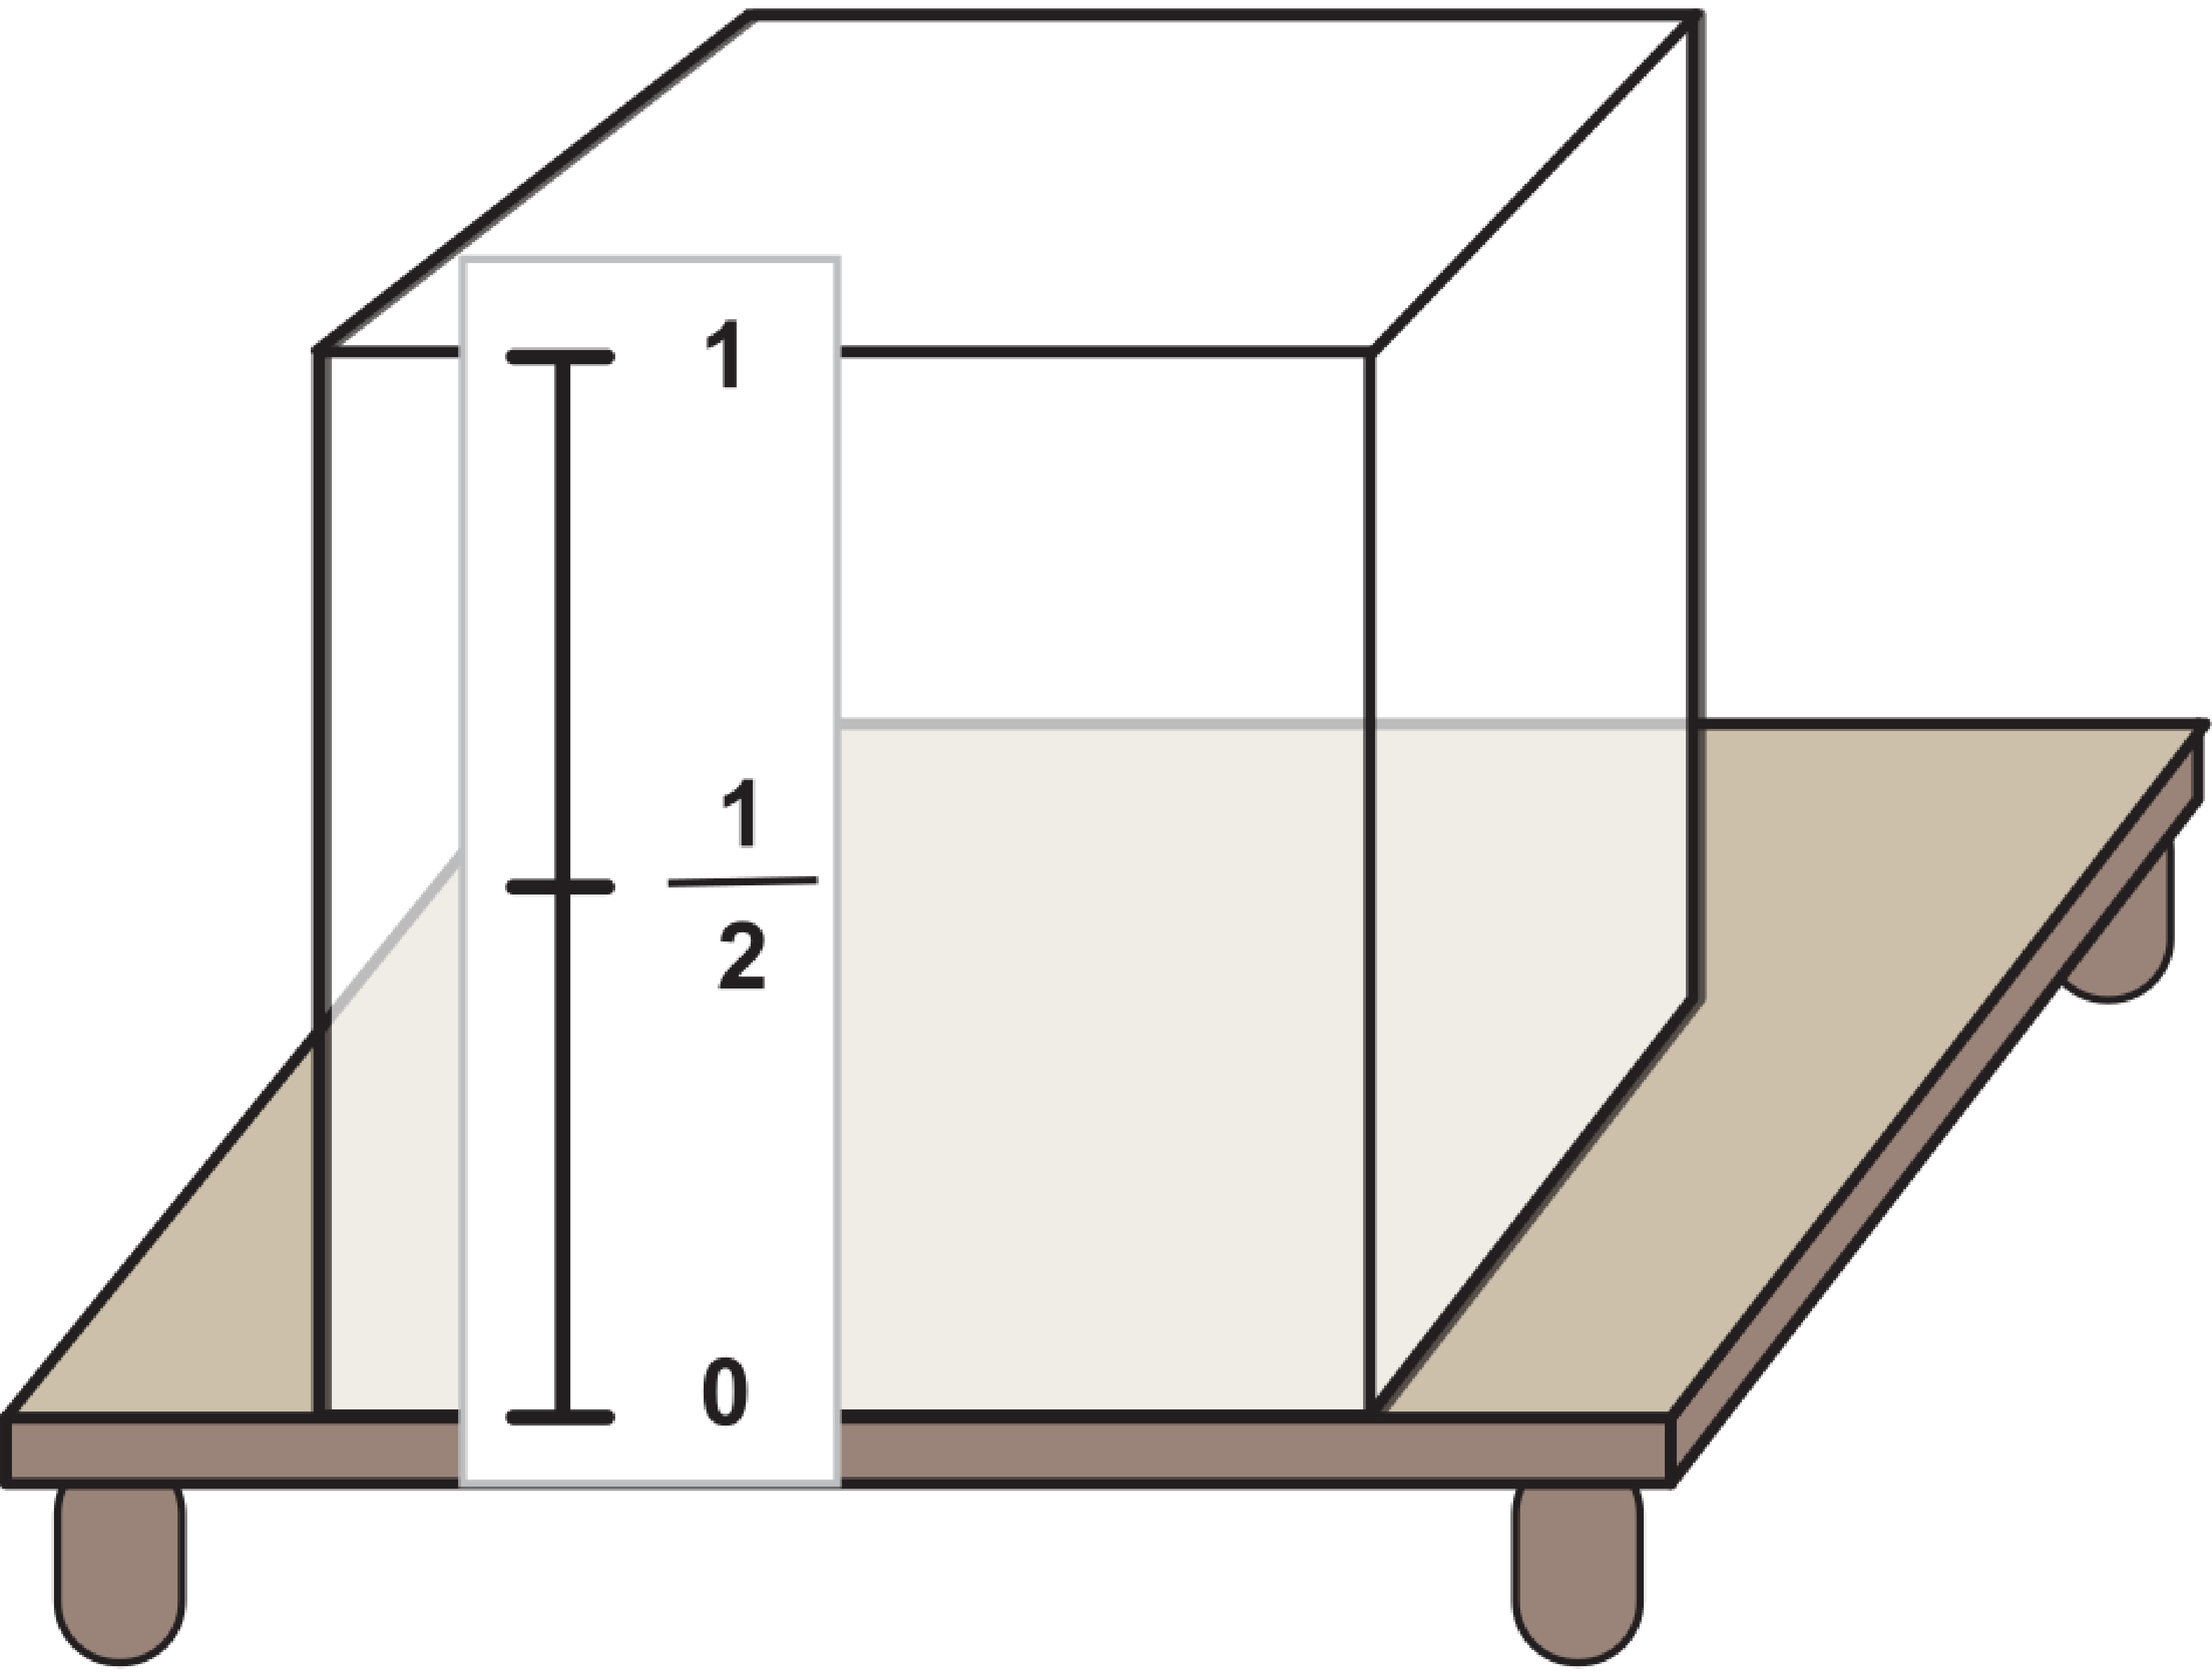
\includegraphics[width=145pt, keepaspectratio]{../figuras/licao03/ativ1_fig09.png}
 %  \end{tabular}
 %  \end{center}
\end{atividade}

\begin{atividade}{}

Use a reta numérica para fazer o que é pedido nos itens a seguir.
\vspace{.2cm}

\begin{center}
\begin{tikzpicture}[x=20mm,y=10mm]
\draw[->] (-1,0) -- (6,0) ; %edit here for the axis
\foreach \x in  {0,1,...,5} % edit here for the vertical lines
\draw[shift={(\x,0)},color=black] (0,3pt) -- (0pt,-3pt)
node[below] {$\x$};

\foreach \x in  {0.25,0.5,...,4.75} % edit here for the vertical lines
\draw[shift={(\x,0)},color=black] (0,2pt) -- (0pt,-2pt);
\end{tikzpicture}
\end{center}

\begin{enumerate} [\quad a)] %s
\item    Marque os pontos que representam as quantidades de pizza nos casos (A), (B) e (C) a seguir.
  
\begin{center}
\begin{tabular}{>{\centering\arraybackslash}m{.2\textwidth} >{\centering\arraybackslash}m{.35\textwidth} >{\centering\arraybackslash}m{.35\textwidth}}


(A) & (B) & (C) \\
{\parbox[c][130pt][c]{80pt}{\null\vfill
\centering

\includegraphics[width=55pt, keepaspectratio]{../figuras/licao03/pizza.png}
\vfill\null}}
&
{\parbox[c][130pt][c]{130pt}{\null\vfill
\centering

\includegraphics[width=55pt, keepaspectratio]{../figuras/licao03/pizza.png} 
\includegraphics[width=55pt, keepaspectratio]{../figuras/licao03/pizza.png}
\vfill\null}}
&
{\begin{tabular}{cc}

\includegraphics[width=55pt, keepaspectratio]{../figuras/licao03/pizza.png}
& 
\includegraphics[width=55pt, keepaspectratio]{../figuras/licao03/pizza.png}\\

\includegraphics[width=55pt, keepaspectratio]{../figuras/licao03/pizza.png} & 
\includegraphics[width=55pt, keepaspectratio]{../figuras/licao03/pizza.png}
\end{tabular}}
\end{tabular}
\end{center}

\item  E agora, que pontos na reta numérica representam as quantidades de pizza dos casos (D), (E), (F) e (G)? 
\end{enumerate} 

\begin{center}
\begin{tabular}{ccccccc}
(D)&\quad\quad\quad & (E) &\quad\quad\quad&  (F) &\quad\quad\quad&  (G) \\
 
\includegraphics[width=55pt, keepaspectratio]{../figuras/licao03/ativ2_fig_b_meia_pizza.png} & & 
\includegraphics[width=55pt, keepaspectratio]{../figuras/licao03/ativ2_fig_b_quarto_pizza.png} & &
\includegraphics[width=55pt, keepaspectratio]{../figuras/licao03/ativ2_fig_b_tres_quartos_pizza.png} & &
\includegraphics[width=55pt, keepaspectratio]{../figuras/licao03/pizza.png}
\includegraphics[width=55pt, keepaspectratio]{../figuras/licao03/ativ2_fig_b_meia_pizza.png}
\end{tabular}
\end{center}

% \begin{center}
% \begin{tikzpicture}[x=30mm,y=30mm]
% \draw[->] (-1/4,0) -- (2.5,0) ; %edit here for the axis
% \foreach \x in  {0,0.25,...,2} % edit here for the vertical lines
% \draw[shift={(\x,0)},color=black] (0,3pt) -- (0pt,-3pt);
% \foreach \x in  {0,1,2}
% \draw[shift={(\x,0)},color=black] (0,3pt) -- (0pt,-3pt) node[below] {$\x$};
% \end{tikzpicture}
% \end{center}
\end{atividade}

\begin{atividade}{}

Para cada uma das figuras a seguir, marque na reta numérica o ponto correspondente à fração da unidade destacada na imagem:


\begin{enumerate} [\quad a)] %s

\item A unidade é o lápis maior.

\begin{center}

\includegraphics[width=50.25mm, keepaspectratio]{../figuras/licao03/ativ4_fig_a0.png}
\quad\quad\quad \begin{tikzpicture}[x=49.25mm,y=56.25mm]
\draw[->] (-0.3,0) -- (1.3,0) ; %edit here for the axis
\foreach \x in  {0,1} % edit here for the vertical lines
\draw[shift={(\x,0)},color=black] (0,3pt) -- (0pt,-3pt)
node[below] {$\x$};
\draw[shift={(.5,0)},color=black] (0,3pt) -- (0pt,-3pt)
node[below] {$\frac{1}{2}$};
\end{tikzpicture}
\end{center}

\item     A unidade é uma pizza.

\begin{center}
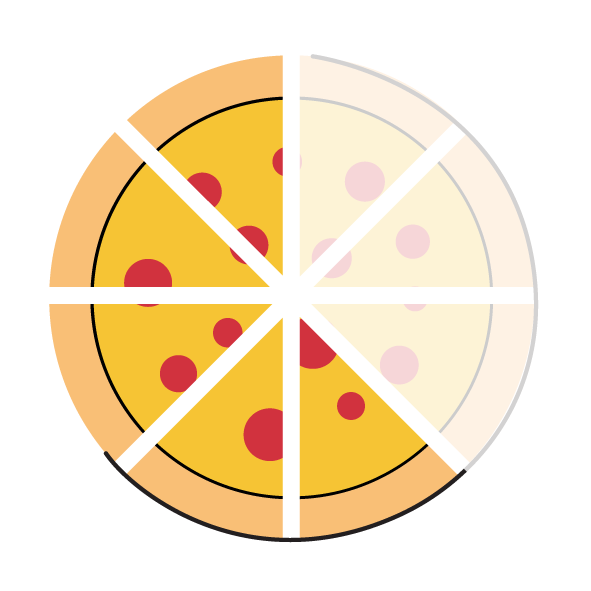
\includegraphics[width=60pt, keepaspectratio]{../figuras/licao03/ativ4_fig_a.png}
\quad\quad\quad \begin{tikzpicture}[x=56.25mm,y=56.25mm]
\draw[->] (-0.3,0) -- (1.3,0) ; %edit here for the axis
\foreach \x in  {0,1} % edit here for the vertical lines
\draw[shift={(\x,0)},color=black] (0,3pt) -- (0pt,-3pt)
node[below] {$\x$};

\foreach \x in {1,...,7}
\draw[shift={(\x/8,0)},color=black] (0,3pt) -- (0pt,-3pt);
\foreach \x in {1,3,5,7}
\node[below] at (\x/8,-3pt) {$\frac{\x}{8}$};
\end{tikzpicture}
\end{center}
%\newpage
\item     A unidade é uma barra de chocolate.

\begin{center}
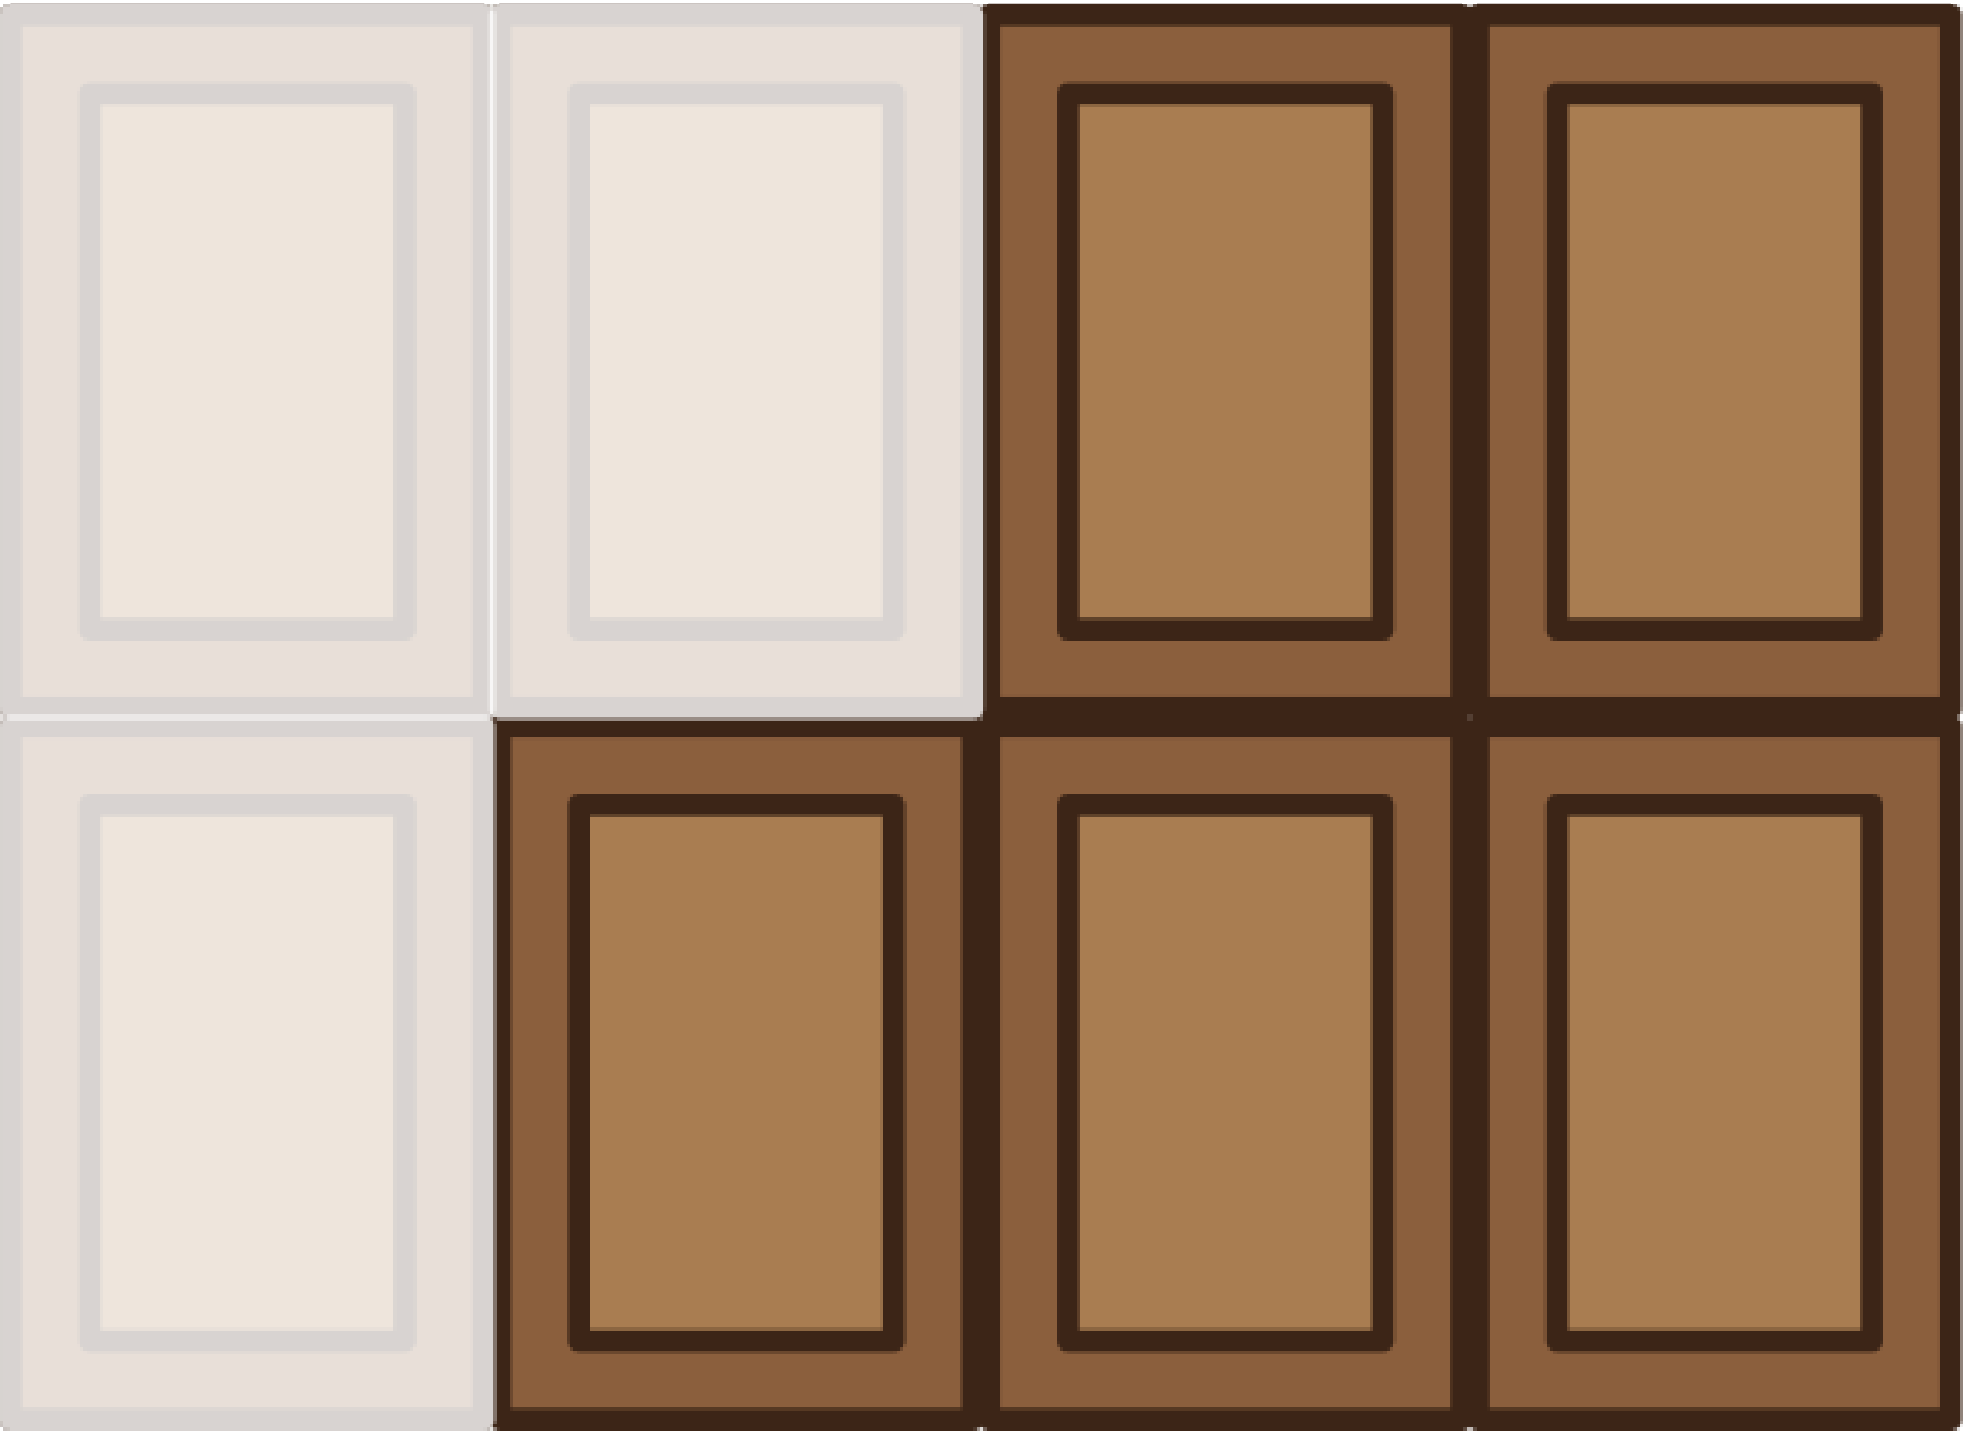
\includegraphics[width=100pt, keepaspectratio]{../figuras/licao03/ativ4_fig_b.png} \quad \quad \quad
\begin{tikzpicture}[x=56.25mm,y=56.25mm]
\draw[->] (-0.3,0) -- (1.3,0) ; %edit here for the axis
\foreach \x in  {0,1} % edit here for the vertical lines
\draw[shift={(\x,0)},color=black] (0,3pt) -- (0pt,-3pt)
node[below] {$\x$};

\foreach \x in {1,...,7}
\draw[shift={(\x/8,0)},color=black] (0,3pt) -- (0pt,-3pt);

\foreach \x in {2,4,6}
\node[below] at (\x/8,-3pt) {$\frac{\x}{8}$};
\end{tikzpicture}
\end{center}

\item     A unidade é uma maçã.

\begin{center}

\includegraphics[width=70pt, keepaspectratio]{../figuras/licao03/ativ4_fig_c.png} \quad \quad \quad
\begin{tikzpicture}[x=60mm,y=60mm]
\draw[->] (-1/4,0) -- (1+1/4,0) ; %edit here for the axis
\foreach \x in  {0,0.25,...,1}{ % edit here for the vertical lines
\draw[shift={(\x,0)},color=black] (0,3pt) -- (0pt,-3pt);}
\foreach \x in  {0,1}
\draw[shift={(\x,0)},color=black] (0,3pt) -- (0pt,-3pt) node[below] {$\x$};
\foreach \x in  {1,2, 3}
\draw[shift={(\x/4,0)},color=black] (0,3pt) -- (0pt,-3pt) node[below] {$\frac{\x}{4}$};
\end{tikzpicture}
\end{center}

  \item     A unidade é um sanduíche de queijo com presunto.

\begin{center}
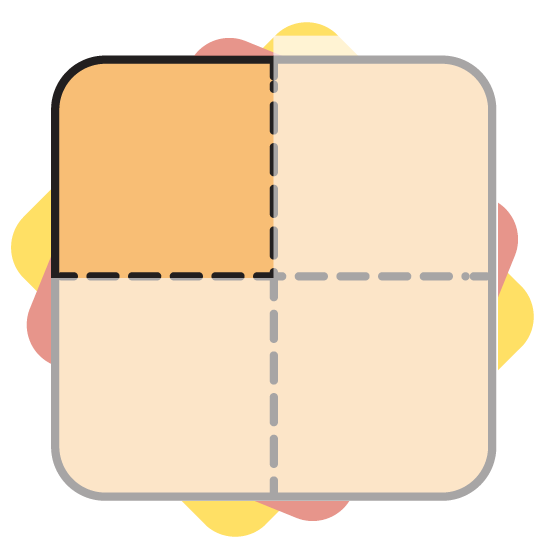
\includegraphics[width=80pt, keepaspectratio]{../figuras/licao03/ativ4_fig_d2.png} \quad \quad \quad
\begin{tikzpicture}[x=60mm,y=60mm]
\draw[->] (-1/4,0) -- (1+1/4,0) ; %edit here for the axis
\foreach \x in  {0,0.25,...,1}{ % edit here for the vertical lines
\draw[shift={(\x,0)},color=black] (0,3pt) -- (0pt,-3pt);}
\foreach \x in  {0,1}
\draw[shift={(\x,0)},color=black] (0,3pt) -- (0pt,-3pt) node[below] {$\x$};
\foreach \x in  {1,3}
\draw[shift={(\x/4,0)},color=black] (0,3pt) -- (0pt,-3pt) node[below] {$\frac{\x}{4}$};
\draw[shift={(.5,0)},color=black] (0,3pt) -- (0pt,-3pt) node[below] {$\frac{1}{2}$};
\end{tikzpicture}
\end{center}

\item A unidade é uma torta.\begin{center}
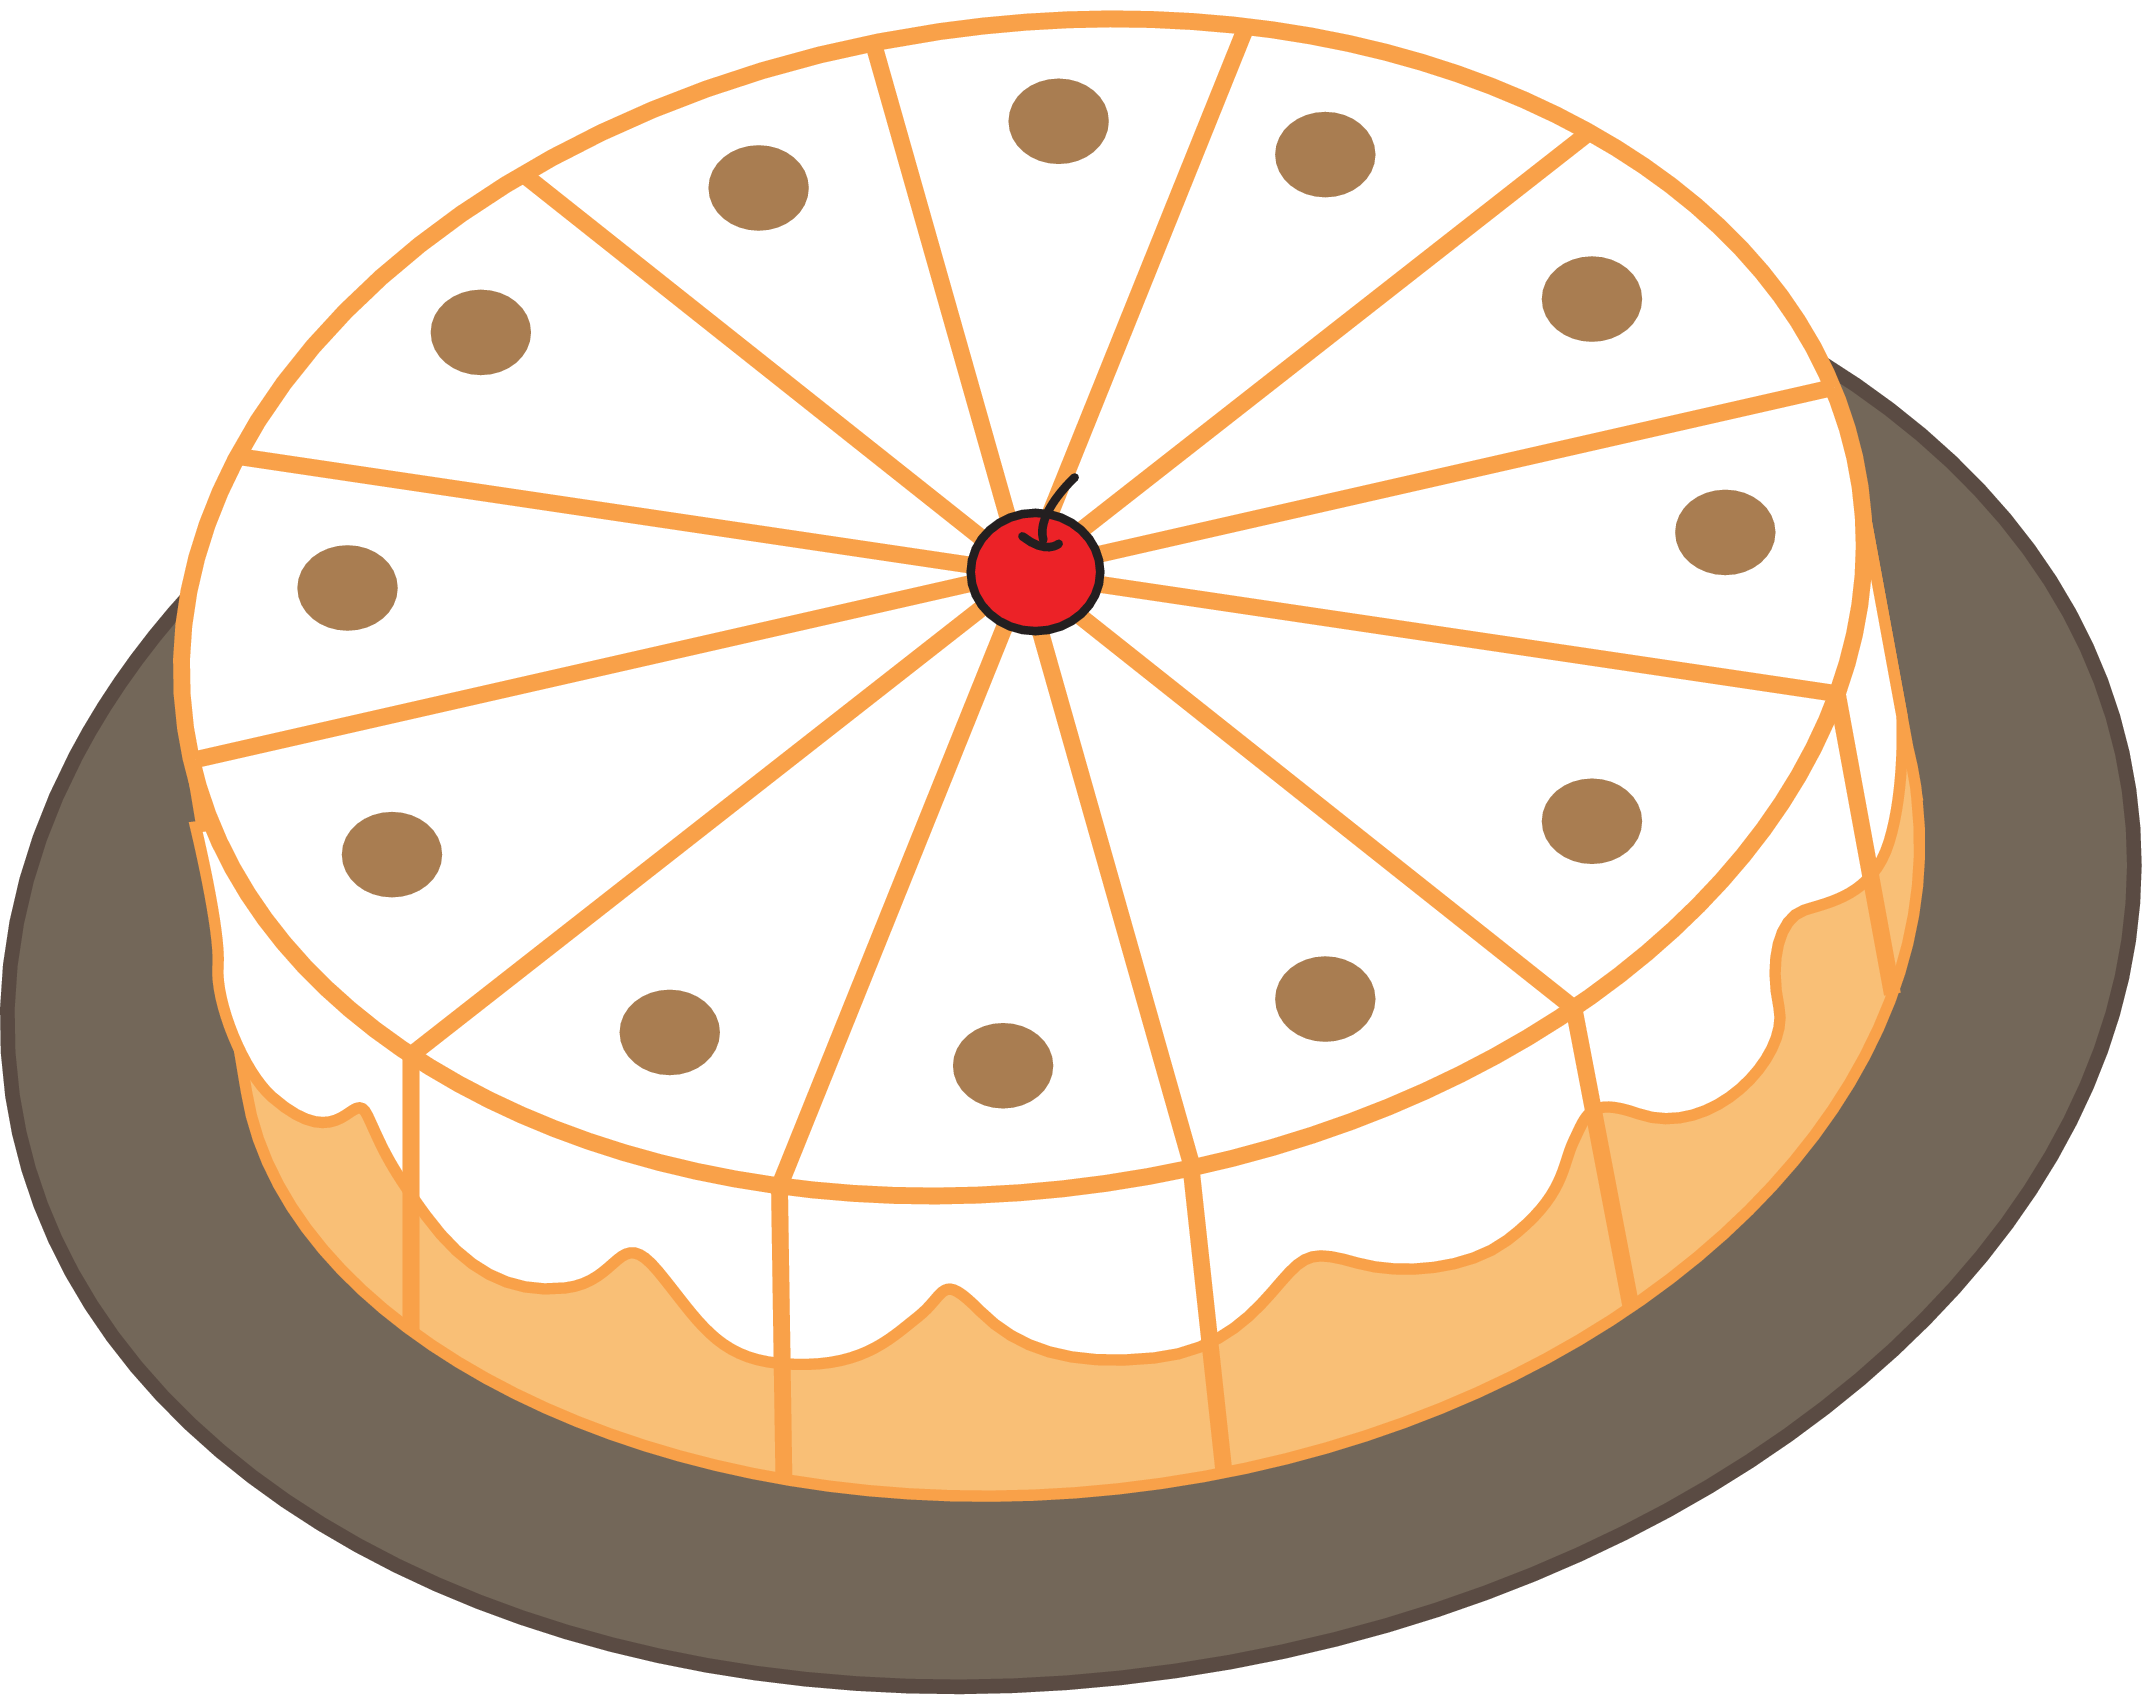
\includegraphics[width=100pt, keepaspectratio]{../figuras/licao03/ativ4_fig_e.png} \quad \quad \quad
 \begin{tikzpicture}[x=50.71mm,y=25.71mm]
\draw[->] (-.2,0) -- (1.3,0) ; %edit here for the axis
\foreach \x in  {0,0.083,...,1}{ % edit here for the vertical lines
\draw[shift={(\x,0)},color=black] (0,3pt) -- (0pt,-3pt);}
\foreach \x in  {0,1}
\node[below] at (\x,-3pt) {$\x$};
\foreach \x in  {3,9}
\node[below] at (\x/12,-3pt)  {$\frac{\x}{12}$};
\node[below] at (.5,-3pt)  {$\frac{1}{2}$};
\end{tikzpicture}
\end{center}

  \item     A unidade é um biscoito.

\begin{center}

\includegraphics[width=100pt, keepaspectratio]{../figuras/licao03/ativ4_fig_f.png} \quad \quad
\begin{tikzpicture}[x=22.71mm,y=25.71mm]
\draw[->] (-.3,0) -- (3.3,0) ; %edit here for the axis
\foreach \x in  {0,0.5,...,3}{ % edit here for the vertical lines
\draw[shift={(\x,0)},color=black] (0,3pt) -- (0pt,-3pt);}
\foreach \x in  {0,1,2,3}
\draw[shift={(\x,0)},color=black] (0,3pt) -- (0pt,-3pt) node[below] {$\x$};
\foreach \x in  {1,3,5}
\draw[shift={(\x/2,0)},color=black] (0,3pt) -- (0pt,-3pt) node[below] {$\frac{\x}{2}$};
\end{tikzpicture}
\end{center}

  \item     A unidade é um copo cheio.
\end{enumerate} %s

\begin{flushright}
 \begin{tabular}{rcr}

\includegraphics[width=50pt, keepaspectratio]{../figuras/licao03/ativ4_fig_g.png}  & \quad\quad\quad\quad&
 \begin{tikzpicture}[x=25.71mm,y=25.71mm]
\draw[->] (-.5,0) -- (3,0) ; %edit here for the axis
\foreach \x in  {0,0.5,...,2.5}{ % edit here for the vertical lines
\draw[shift={(\x,0)},color=black] (0,3pt) -- (0pt,-3pt);}
\foreach \x in  {0,1,2}
\draw[shift={(\x,0)},color=black] (0,3pt) -- (0pt,-3pt) node[below] {$\x$};
\foreach \x in  {1,3,5}
\draw[shift={(\x/2,0)},color=black] (0,3pt) -- (0pt,-3pt) node[below] {$\frac{\x}{2}$};
\end{tikzpicture}
\end{tabular}
\end{flushright}
\end{atividade}

\begin{atividade}{}
  Que fração da figura está pintada de vermelho? Ligue cada figura ao número correspondente  destacado na reta numérica.
  
\begin{longtable}{lccc}
%retangulos
a)& Figura A & & Figura B\\
& \begin{tikzpicture}[x=30mm,y=30mm,scale=.6]
  \draw[ fill=attention] (-1.8,0) rectangle (0,1.2);
 % \node [above] at (-.9,1.2) {Figura 1};
\end{tikzpicture}
&&

\begin{tikzpicture}[x=30mm,y=30mm,scale=.6]
\draw[fill=common, fill opacity=.3] (0,0) rectangle (1.8,1.2);
%\node [above] at (.9,1.2) {Figura 2};
\draw[fill=attention] (0,0) -- (0,1.2) --(1.8,0)--cycle;
\end{tikzpicture}

\\

\multicolumn{4}{c}{
\parbox[c][.7cm][t]{8cm}{ } }

\\

&\multicolumn{3}{c}{
\begin{tikzpicture}[x=45mm,y=45mm]
\draw[->] (-0.5,0) -- (1.5,0) ; %edit here for the axis
\foreach \x in  {0,1} % edit here for the vertical lines
\draw[shift={(\x,0)},color=black] (0,3pt) -- (0pt,-3pt)
node[below] {$\x$};
\draw[shift={(0.5,0)},color=black] (0,3pt) -- (0pt,-3pt)
node[below] {$\frac{1}{2}$};
\end{tikzpicture}
}

\\
% item b)
b)& Figura A & & Figura B \\
 %triangulos
& \begin{tikzpicture}[x=30mm,y=30mm]
\def\scale{.6}% to rescale the polygons only.

\foreach \x in {90,210,330}{
\draw[attention,fill=attention, shift={(0,0.6)}, scale=\scale] (\x:0.7) -- (\x + 120: 0.7) -- (0,0)--cycle;
\draw[shift={(0,0.6)}, scale=\scale] (\x:0.7) -- (\x + 120: 0.7);}
\draw[shift={(0,0.6)}, scale=\scale] (-90:0.35) -- (30: 0.35) -- (150: 0.35) -- cycle;
 %\node [above] at (-.9,1.2) {Figura 1};
\end{tikzpicture}
&&
\begin{tikzpicture}[x=30mm,y=30mm]
\def\scale{.6}% to rescale the polygons only.
\fill[shift={(1,0.6)}, scale=\scale, common, fill opacity=.3] (90:0.7) -- (210: 0.7)--(330:.7)--cycle;
\foreach \x in {90,210,330}{
\draw[shift={(1,0.6)}, scale=\scale] (\x:0.7) -- (\x + 120: 0.7);}
\draw[fill=attention, shift={(1,0.6)}, scale=\scale] (-90:0.35) -- (30: 0.35) -- (150: 0.35) -- cycle;
% \node [above] at (.9,1.2) {Figura 2};
\end{tikzpicture}

\\

\multicolumn{4}{c}{
\parbox[c][.7cm][t]{8cm}{ } }

\\
&\multicolumn{3}{c}{
\begin{tikzpicture}[x=60mm,y=60mm]
\draw[->] (-1/4,0) -- (1+1/4,0) ; %edit here for the axis
\foreach \x in  {0,0.25,...,1}{ % edit here for the vertical lines
\draw[shift={(\x,0)},color=black] (0,3pt) -- (0pt,-3pt);}
\foreach \x in  {0,1}
\draw[shift={(\x,0)},color=black] (0,3pt) -- (0pt,-3pt) node[below] {$\x$};
\foreach \x in  {1,3}
\draw[shift={(\x/4,0)},color=black] (0,3pt) -- (0pt,-3pt) node[below] {$\frac{\x}{4}$};
\end{tikzpicture}}
\\
\clearpage

c) & Figura A & & Figura B \\

%quadrados


& \begin{tikzpicture}[x=30mm,y=30mm]
\def\scale{.6}
%
\draw[fill=common, fill opacity=.3, scale=\scale] (-1.2,0) rectangle (0,1.2);
\draw[fill=attention, scale=\scale] (-1.2,0) rectangle (-0.8,.4);
\draw[fill=attention, scale=\scale] (-.4,0) rectangle (0,.4);
\draw[fill=attention, scale=\scale] (-1.2,0.8) rectangle (-0.8,1.2);
\draw[fill=attention, scale=\scale] (-.4,0.8) rectangle (0,1.2);
\draw[fill=attention, scale=\scale] (-.8,0.4) rectangle (-0.4,.8);

% \draw[ fill=attention, scale=\scale] (-1.2,.8) rectangle (0,1.2);

% \draw[fill=common, fill opacity=.3, scale=\scale] (-0.8,0) rectangle (-.4,.4);
% \draw[ fill=attention, scale=\scale] (-0.8,.4) rectangle (-0.4,.8);
% \draw[fill=common, fill opacity=.3, scale=\scale] (-0.8,.8) rectangle (-.4,1.2);
\end{tikzpicture}
&&
 \begin{tikzpicture}[x=30mm,y=30mm]
\def\scale{.6}
\draw[fill=attention, scale=\scale] (0,0) rectangle (1.2,1.2);
\end{tikzpicture}

\\

\multicolumn{4}{c}{
\parbox[c][.7cm][t]{8cm}{ } }

\\

&\multicolumn{3}{c}{
\begin{tikzpicture}[x=45mm,y=45mm]
\draw[->] (-0.5,0) -- (1.5,0) ; %edit here for the axis
\foreach \x in  {0,0.1111,...,1}{ % edit here for the vertical lines
\draw[shift={(\x,0)},color=black] (0,3pt) -- (0pt,-3pt);}
\foreach \x in  {0,1}
\draw[shift={(\x,0)},color=black] (0,3pt) -- (0pt,-3pt) node[below] {$\x$};
\foreach \x in  {4,5}
\draw[shift={(\x/9,0)},color=black] (0,3pt) -- (0pt,-3pt) node[below] {$\frac{\x}{9}$};
\end{tikzpicture}}
\\

%hexagonos
d) & Figura A & & Figura B \\

& \begin{tikzpicture}[x=30mm,y=30mm]
\def\scale{.6}% to rescale the polygons only.

%hexagon on the left
\fill[shift={(0,0.6)}, fill=attention, scale=\scale] (0,0) -- (90:0.7) -- (150:0.7)-- (210:.7);
\fill[shift={(0,0.6)}, fill=common, fill opacity=.3, scale=\scale] (0,0) -- (90:0.7) -- (30:0.7)-- (-30:.7) -- (-90:.7) -- (-150:.7)--cycle;
\foreach \x in {30,90,...,330}{
\draw[shift={(0,0.6)}, scale=\scale] (\x:0.7) -- (\x + 60: 0.7);
\draw[shift={(0,0.6)}, scale=\scale] (0,0) -- (\x:0.7);}
\end{tikzpicture}
&&
\begin{tikzpicture}[x=30mm,y=30mm]
\def\scale{.6}% to rescale the polygons only.

%hexagon on the right
\foreach \x in {30,90,...,330}{
\draw[shift={(1,0.6)}, fill=attention,attention, scale=\scale] (\x:0.7) -- (\x + 60: 0.7) --(0,0) --cycle;
\draw[shift={(1,0.6)}, fill=attention, scale=\scale] (\x:0.7) -- (\x + 60: 0.7);}
\end{tikzpicture}

\\

\multicolumn{4}{c}{
\parbox[c][.7cm][t]{8cm}{ } }

\\
&\multicolumn{3}{c}{
\begin{tikzpicture}[x=68mm,y=68mm]
\draw[->] (-1/6,0) -- (1+1/6,0) ; %edit here for the axis
\foreach \x in  {0,0.1667,...,1}{ % edit here for the vertical lines
\draw[shift={(\x,0)},color=black] (0,3pt) -- (0pt,-3pt);}
\foreach \x in  {0,1}
\draw[shift={(\x,0)},color=black] (0,3pt) -- (0pt,-3pt) node[below] {$\x$};
\foreach \x in  {1,2}
\draw[shift={(\x/3,0)},color=black] (0,3pt) -- (0pt,-3pt) node[below] {$\frac{\x}{3}$};
\end{tikzpicture} }
\\

e) & Figura A & Figura B & Figura C \\

%os baianos e os novos retangulos
& \begin{tikzpicture} [x=30mm,y=30mm]
\def\scalefig {.6}
\draw[shift={(-.35*\scalefig,0.3)}, fill=attention, scale=\scalefig] (-1.5,0) rectangle (-0.5,1.2);
\draw[shift={(-.35*\scalefig,0.3)}, scale=\scalefig, fill=common, fill opacity=.3] (-.5,0) rectangle (0,1.2);
\draw[shift={(-.35*\scalefig,0.3)}, scale=\scalefig] (-1,0) -- (-1,1.2);
\end{tikzpicture}
&
\begin{tikzpicture} [x=30mm,y=30mm]
\def\scalefig {.6}
\draw[shift={(1.25*\scalefig,0.3)}, fill=common, fill opacity=.3, scale=\scalefig] (-1.5,0) rectangle (-1,1.2);
\draw[shift={(1.25*\scalefig,0.3)}, scale=\scalefig, fill=common, fill opacity=.3] (-1,0) rectangle (0,1.2);
\draw[shift={(1.25*\scalefig,0.3)}, scale=\scalefig] (-.5,0) -- (-.5,1.2);
\end{tikzpicture}
&
\begin{tikzpicture} [x=30mm,y=30mm]
\def\scalefig {.6}
\draw[shift={(1.35*\scalefig,0.3)}, fill=attention, scale=\scalefig] (0,0) rectangle (1.5,1.2);
\draw[shift={(1.35*\scalefig,0.3)}, scale=\scalefig] (.5,0) -- (.5,1.2);
\draw[shift={(1.35*\scalefig,0.3)}, scale=\scalefig] (1,0) -- (1,1.2);
\end{tikzpicture}

\\

\multicolumn{4}{c}{
\parbox[c][.7cm][t]{8cm}{ } }

\\
&\multicolumn{3}{c}{
\begin{tikzpicture}[x=55mm,y=55mm]
 \begin{scope}[shift={(-.3,0)}]
\draw[->] (-1/3,0) -- (1.33,0) ; %edit here for the axis
\foreach \x in  {0,1} % edit here for the vertical lines
\draw[shift={(\x,0)},color=black] (0,3pt) -- (0pt,-3pt)
node[below] {$\x$};
\foreach \x in {1,2}
\draw[shift={(\x/3,0)},color=black] (0,3pt) -- (0pt,-3pt)
node[below] {$\frac{\x}{3}$};
\end{scope}
\end{tikzpicture}}
\\

f) & Figura A & Figura B & Figura C \\

&\begin{tikzpicture}[scale=.48]
\fill[common, fill opacity=.3] (0,0) rectangle (45,45);
 \fill[attention] (0,33.75) rectangle (33.75,45);
 \draw[step=11.25, fill=attention] (0,0) grid (45,45);
\end{tikzpicture}
&
\begin{tikzpicture}[scale=.48]
\draw[fill=attention] (0,0) rectangle (45,45);
\end{tikzpicture}
&
\begin{tikzpicture}[scale=.48]
  \draw[fill=common, opacity=.3] (0,0) rectangle (45,45);
%  \draw[step=11.25, fill=white] (0,0) rectangle (45,11.25);
  \draw[fill=attention] (0,0) rectangle (33.75,33.75);
  \draw[step=11.25] (0,0) grid (45,45);
\end{tikzpicture}

\\

\multicolumn{4}{c}{
\parbox[c][.7cm][t]{8cm}{ } }



\\
&\multicolumn{3}{c}{
\begin{tikzpicture}[x=90mm,y=90mm]
 \draw[->] (-1/16,0) -- (1+1/16,0) ; %edit here for the axis
 \foreach \x in  {0,0.0625,...,1}{ % edit here for the vertical lines
 \draw[shift={(\x,0)},color=black] (0,3pt) -- (0pt,-3pt);}
\foreach \x in  {0,1}
\draw[shift={(\x,0)},color=black] (0,3pt) -- (0pt,-3pt) node[below] {$\x$};
\foreach \x in  {3,7,9,13}
\draw[shift={(\x/16,0)},color=black] (0,3pt) -- (0pt,-3pt) node[below] {$\frac{\x}{16}$};
\end{tikzpicture}
}

\end{longtable}

\end{atividade}

\begin{atividade}{}

A faixa a seguir está dividida em 5 partes iguais.

\begin{center}
 \begin{tikzpicture}[x=56.25mm,y=56.25mm]
\foreach \x in {0,1,2,...,4}{
\draw[fill=common, fill opacity=.3] (\x/5,0) rectangle (\x/5 + 1/5,.1);
\draw[step=.2] (0,0) grid (1,.1);
\draw (0,.1)-- (1,.1);}
 \end{tikzpicture}
\end{center}


\begin{enumerate} [\quad a)] %s
  \item    Considerando a faixa como unidade,  complete a reta numérica  escrevendo frações  correspondentes às regiões coloridas em vermelho. 

\begin{center}
  \begin{tikzpicture}[x=56.25mm,y=56.25mm]

\foreach \x in {0,1,2,...,5}{
\fill[fill=common, fill opacity=.3, shift={(0,-\x*.15)}] (\x/5,0) rectangle (1,.1);
\draw[fill=attention, shift={(0,-\x*.15)}] (0,0) rectangle (\x/5,.1);
\draw[step=.2, shift={(0,-\x*.15)}] (0,0) grid (1,.1);
\draw[shift={(0,-\x*.15)}] (0,.1)-- (1,.1);}

\begin{scope}[shift={(0,-.9)}]
\draw[->] (-0.1,0) -- (1.1,0) ; %edit here for the axis
\foreach \x in  {0,1} % edit here for the vertical lines
\draw[shift={(\x,0)},color=black] (0,3pt) -- (0pt,-3pt) node[below] {$\x$};

\foreach \x in  {.2,.4,.6,.8} % edit here for the vertical lines
\draw[shift={(\x,0)},color=black] (0,3pt) -- (0pt,-3pt) node[below] {{\huge $\dfrac{\square}{\square}$}};
\end{scope}

\end{tikzpicture}
 \end{center}

  \item     E as faixas sem pintura vermelha e toda pintada de vermelho? Escreva as frações correspondentes a elas.

\end{enumerate} %s
\end{atividade}

\begin{atividade}{}

A professora Julia pediu que os seus alunos, Pedro e Miguel, marcassem $\frac{1}{2}$ na reta numérica traçada em uma fita, como esta que vocês também receberam:

\begin{center}
 \begin{tikzpicture}[x=56.25mm,y=56.25mm]
\draw[fill=common, fill opacity=.3] (0,-.15) rectangle (1.2,.15);
\draw (0,0) -- (1.2,0) ; %edit here for the axis
\draw (1,3pt) -- (1,-3pt) node[below] {1};
\node at (.03,-.05) {0};
\end{tikzpicture}
\end{center}

Veja as marcações de Pedro e Miguel.

\begin{center}
 \begin{tikzpicture}[x=56.25mm,y=56.25mm]
\draw[fill=common, fill opacity=.3] (0,-.15) rectangle (1.2,.15);
\draw (0,0) -- (1.2,0) ; %edit here for the axis
\draw[dashed] (0.6,-.15) -- (.6,.15);
\draw (1,3pt) -- (1,-3pt) node[below] {1};
\node at (.03,-.05) {0};
\node at (.63,-.05) {$\frac{1}{2}$};

\node at (-.43,0) {Marcação de Pedro};
\draw [->] (-.1,0) -- (-.05,0);

\begin{scope}[yshift=-60]
\draw[fill=common, fill opacity=.3] (0,-.15) rectangle (1.2,.15);
\draw (0,0) -- (1.2,0) ; %edit here for the axis
\draw[dashed] (0.5,-.15) -- (.5,.15);
\draw (1,3pt) -- (1,-3pt) node[below] {1};
\node at (.03,-.05) {0};
\node at (.53,-.05) {$\frac{1}{2}$};

\node at (-.45,0) {Marcação de Miguel};
\draw [->] (-.1,0) -- (-.05,0);
\end{scope}
\end{tikzpicture}
\end{center}

\begin{enumerate} [\quad a)] %s
  \item     É possível ambos estarem corretos? Justifique sua resposta.
  \item     Faça marcações correspondentes a     $\frac{1}{4}$     e a     $\frac{3}{4}$  na reta numérica desenhada na fita que você recebeu. Explique como você fez essas marcações.
  \item     Onde deve ser feita a marcação correspondente a     $\frac{4}{4}$    ?
  \item     E a marcação correspondente a     $\frac{5}{4}$    ?
\end{enumerate} %s
\end{atividade}

\begin{atividade}{}

Um caçador de tesouros encontrou o mapa e o papiro a seguir. Leia as instruções para a localização do tesouro e decida em que local ele deve cavar.

\begin{figure}[H]
\centering

\begin{tikzpicture}[x=1cm,y=1cm, every node/.style={scale=1.10}, scale=1.10]

\node (mapa) at (3,2) {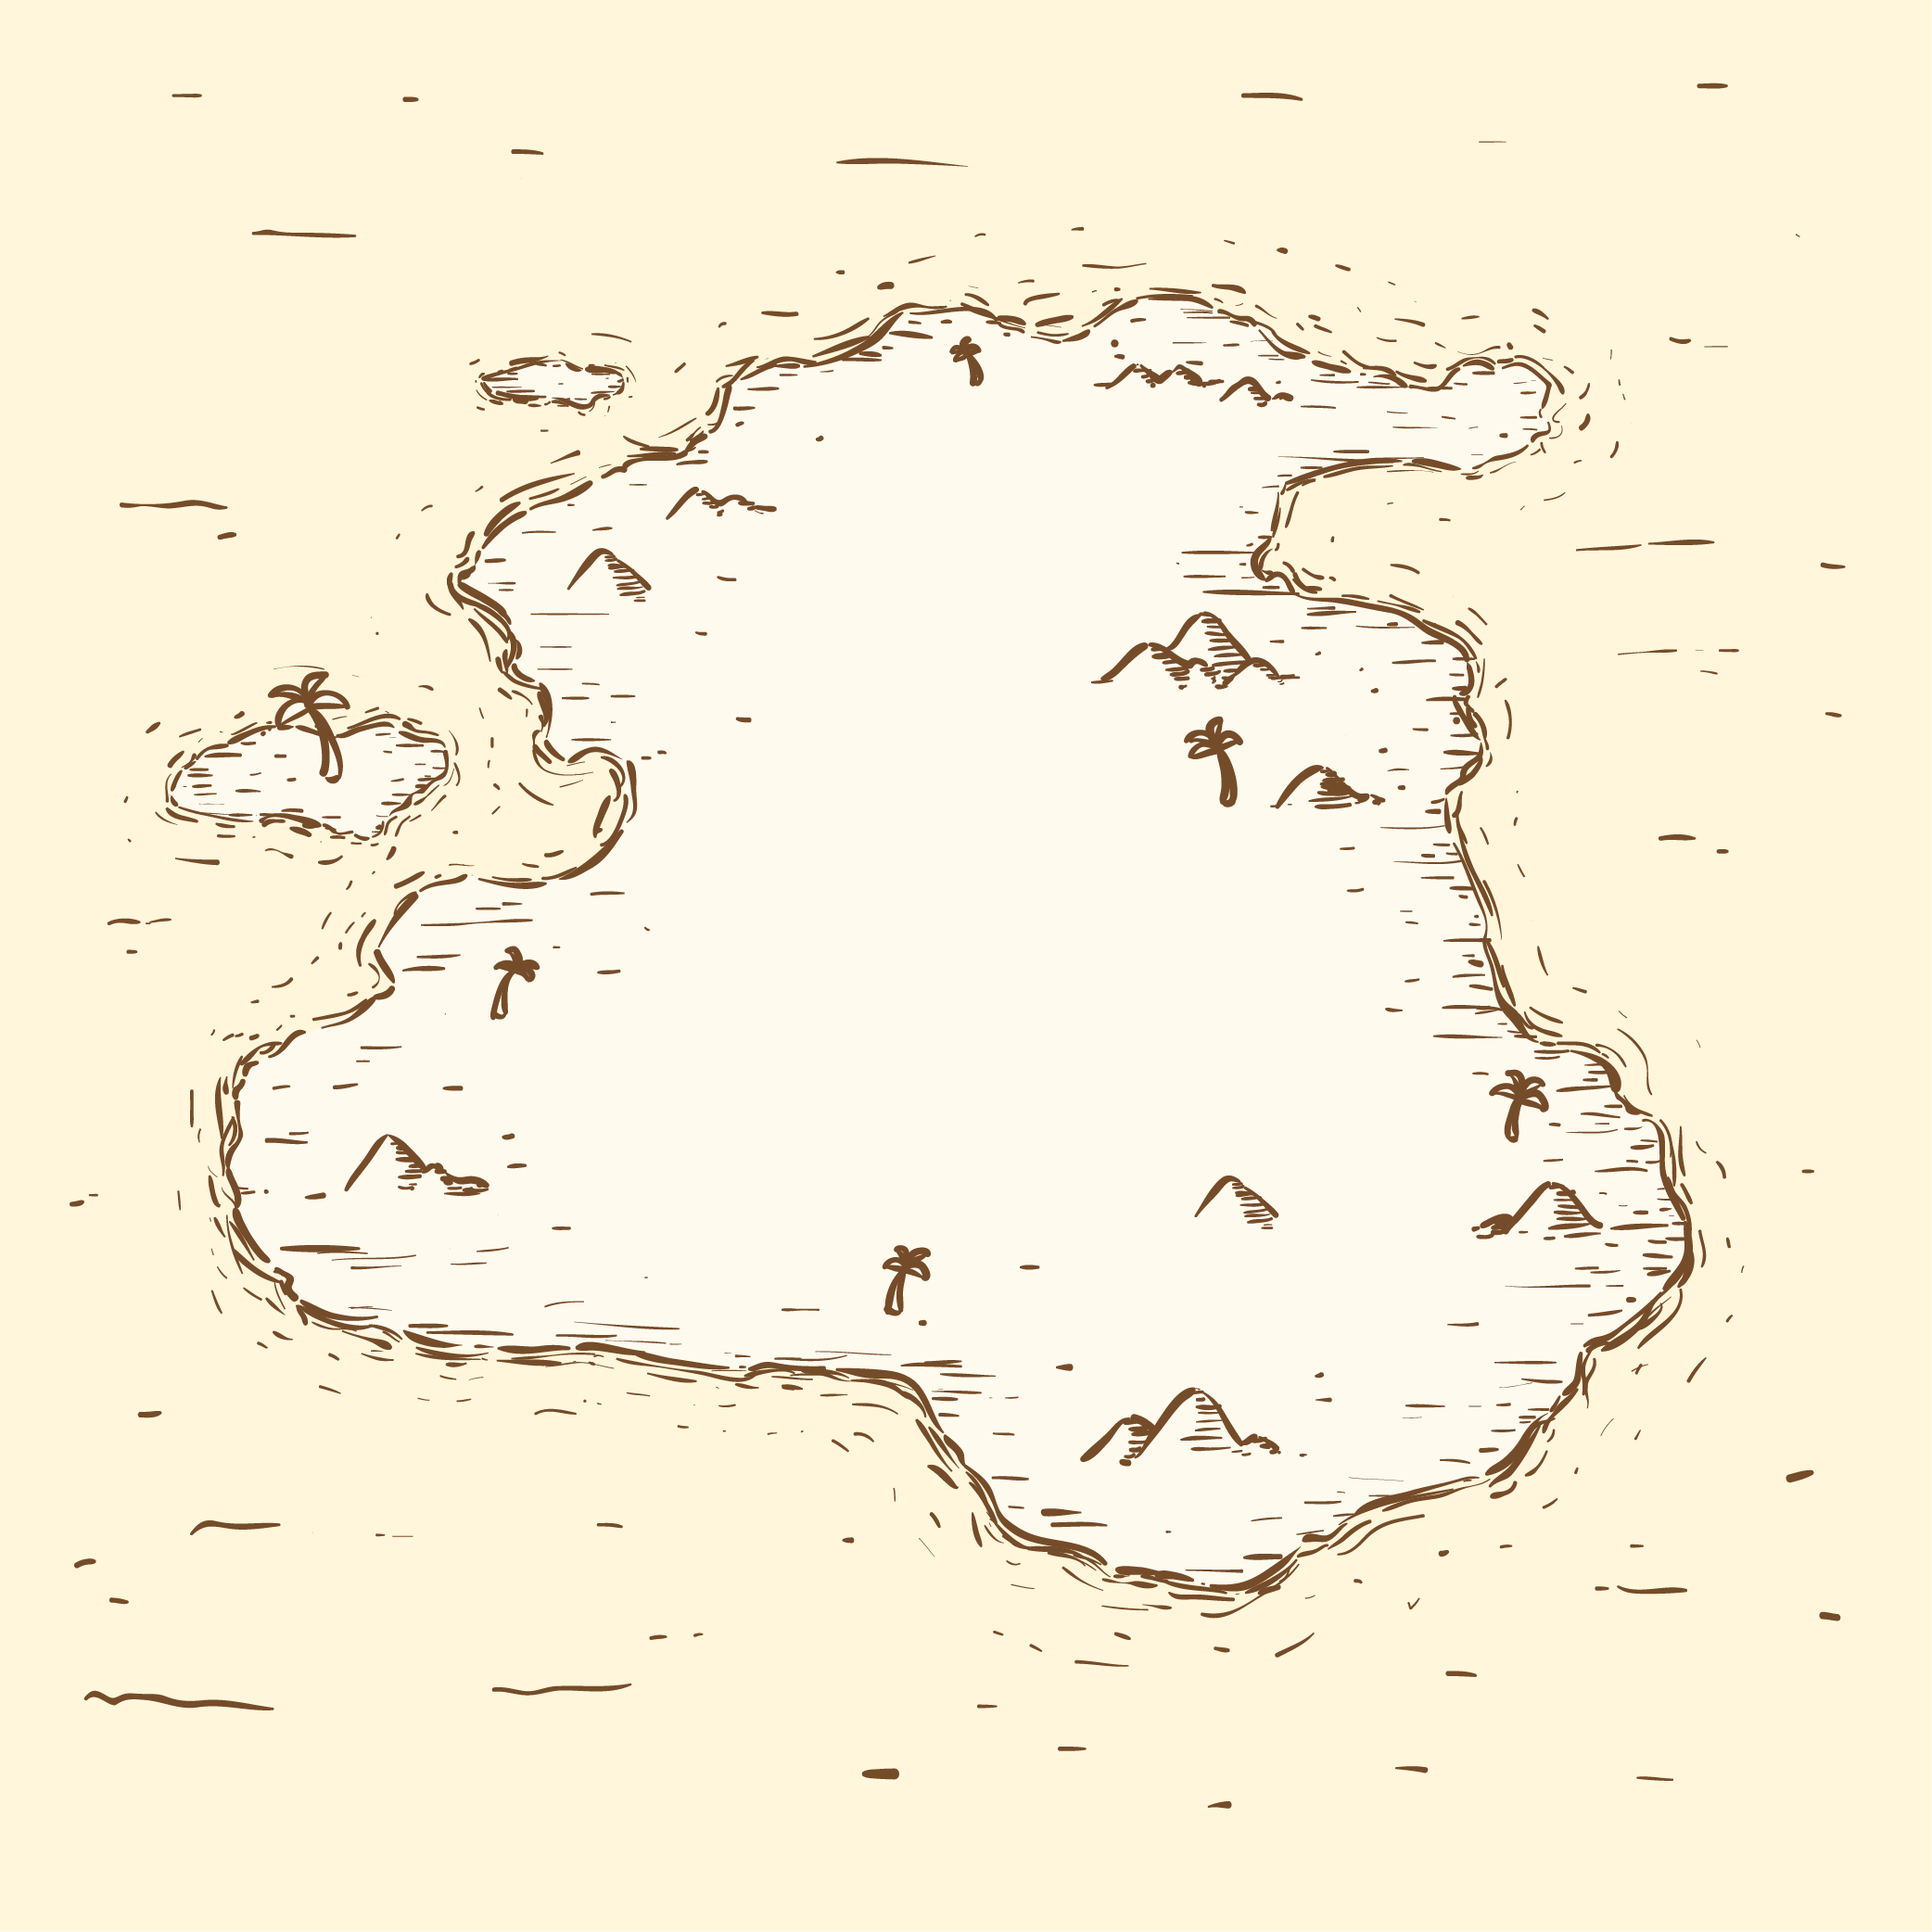
\includegraphics[width=300bp]{../figuras/licao03/mapa.png}};
\node at (.8,0.65) (palm) {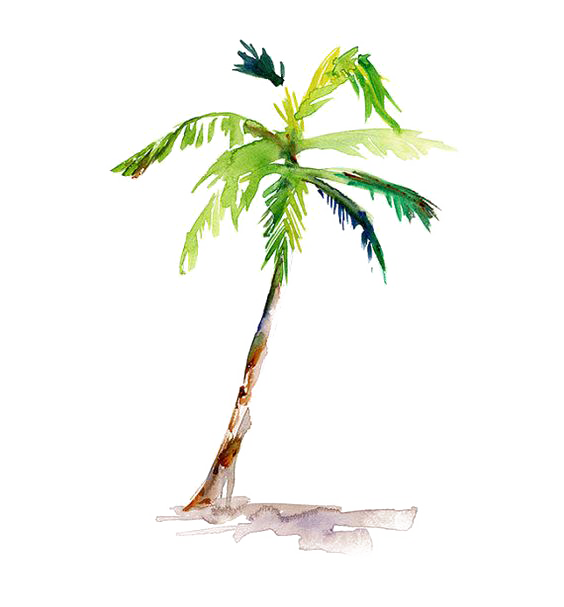
\includegraphics[width=50bp]{../figuras/licao03/palmeira.png}};

\node (pedra) at (4.28,3.85) {
\includegraphics[width=33bp]{../figuras/licao03/pedra.png}};

\draw [dashed] (.85,.1) -- (3.9,3.3);

\draw [ultra thick, red] (3,2) -- (4.5,2);
\end{tikzpicture}

\begin{tikzpicture}
\setlength{\baselineskip}{15pt}
\setlength\parskip{.1em}
\node {
\includegraphics[width=410bp]{../figuras/licao03/papiro.png}};
\node [rectangle]{\parbox{300bp}{
Há dois baús escondidos, um deles carregado com um tesouro. Para localizá-los, você deve seguir o mapa e estas instruções.


\begin{enumerate}[label=\arabic*.,topsep=.5em]
\setlength{\baselineskip}{15pt}
\setlength\parskip{.1em}

\item Use a faixa vermelha como unidade para descobrir a localização dos baús.
\item Os baús estão enterrados no caminho em destaque, alinhados com a palmeira imperial e com a pedra.
\item No mapa, os pontos que marcam os locais em que os baús estão enterrados ficam a $\frac{5}{6}$ e a $\frac{5}{8}$ da unidade, a partir da palmeira. A chave do baú com o tesouro está enterrada a $\frac{13}{8}$ da unidade a partir da palmeira.
\item O baú com o tesouro está mais distante da palmeira.

\end{enumerate}}};
\end{tikzpicture}
\end{figure}

% \noindent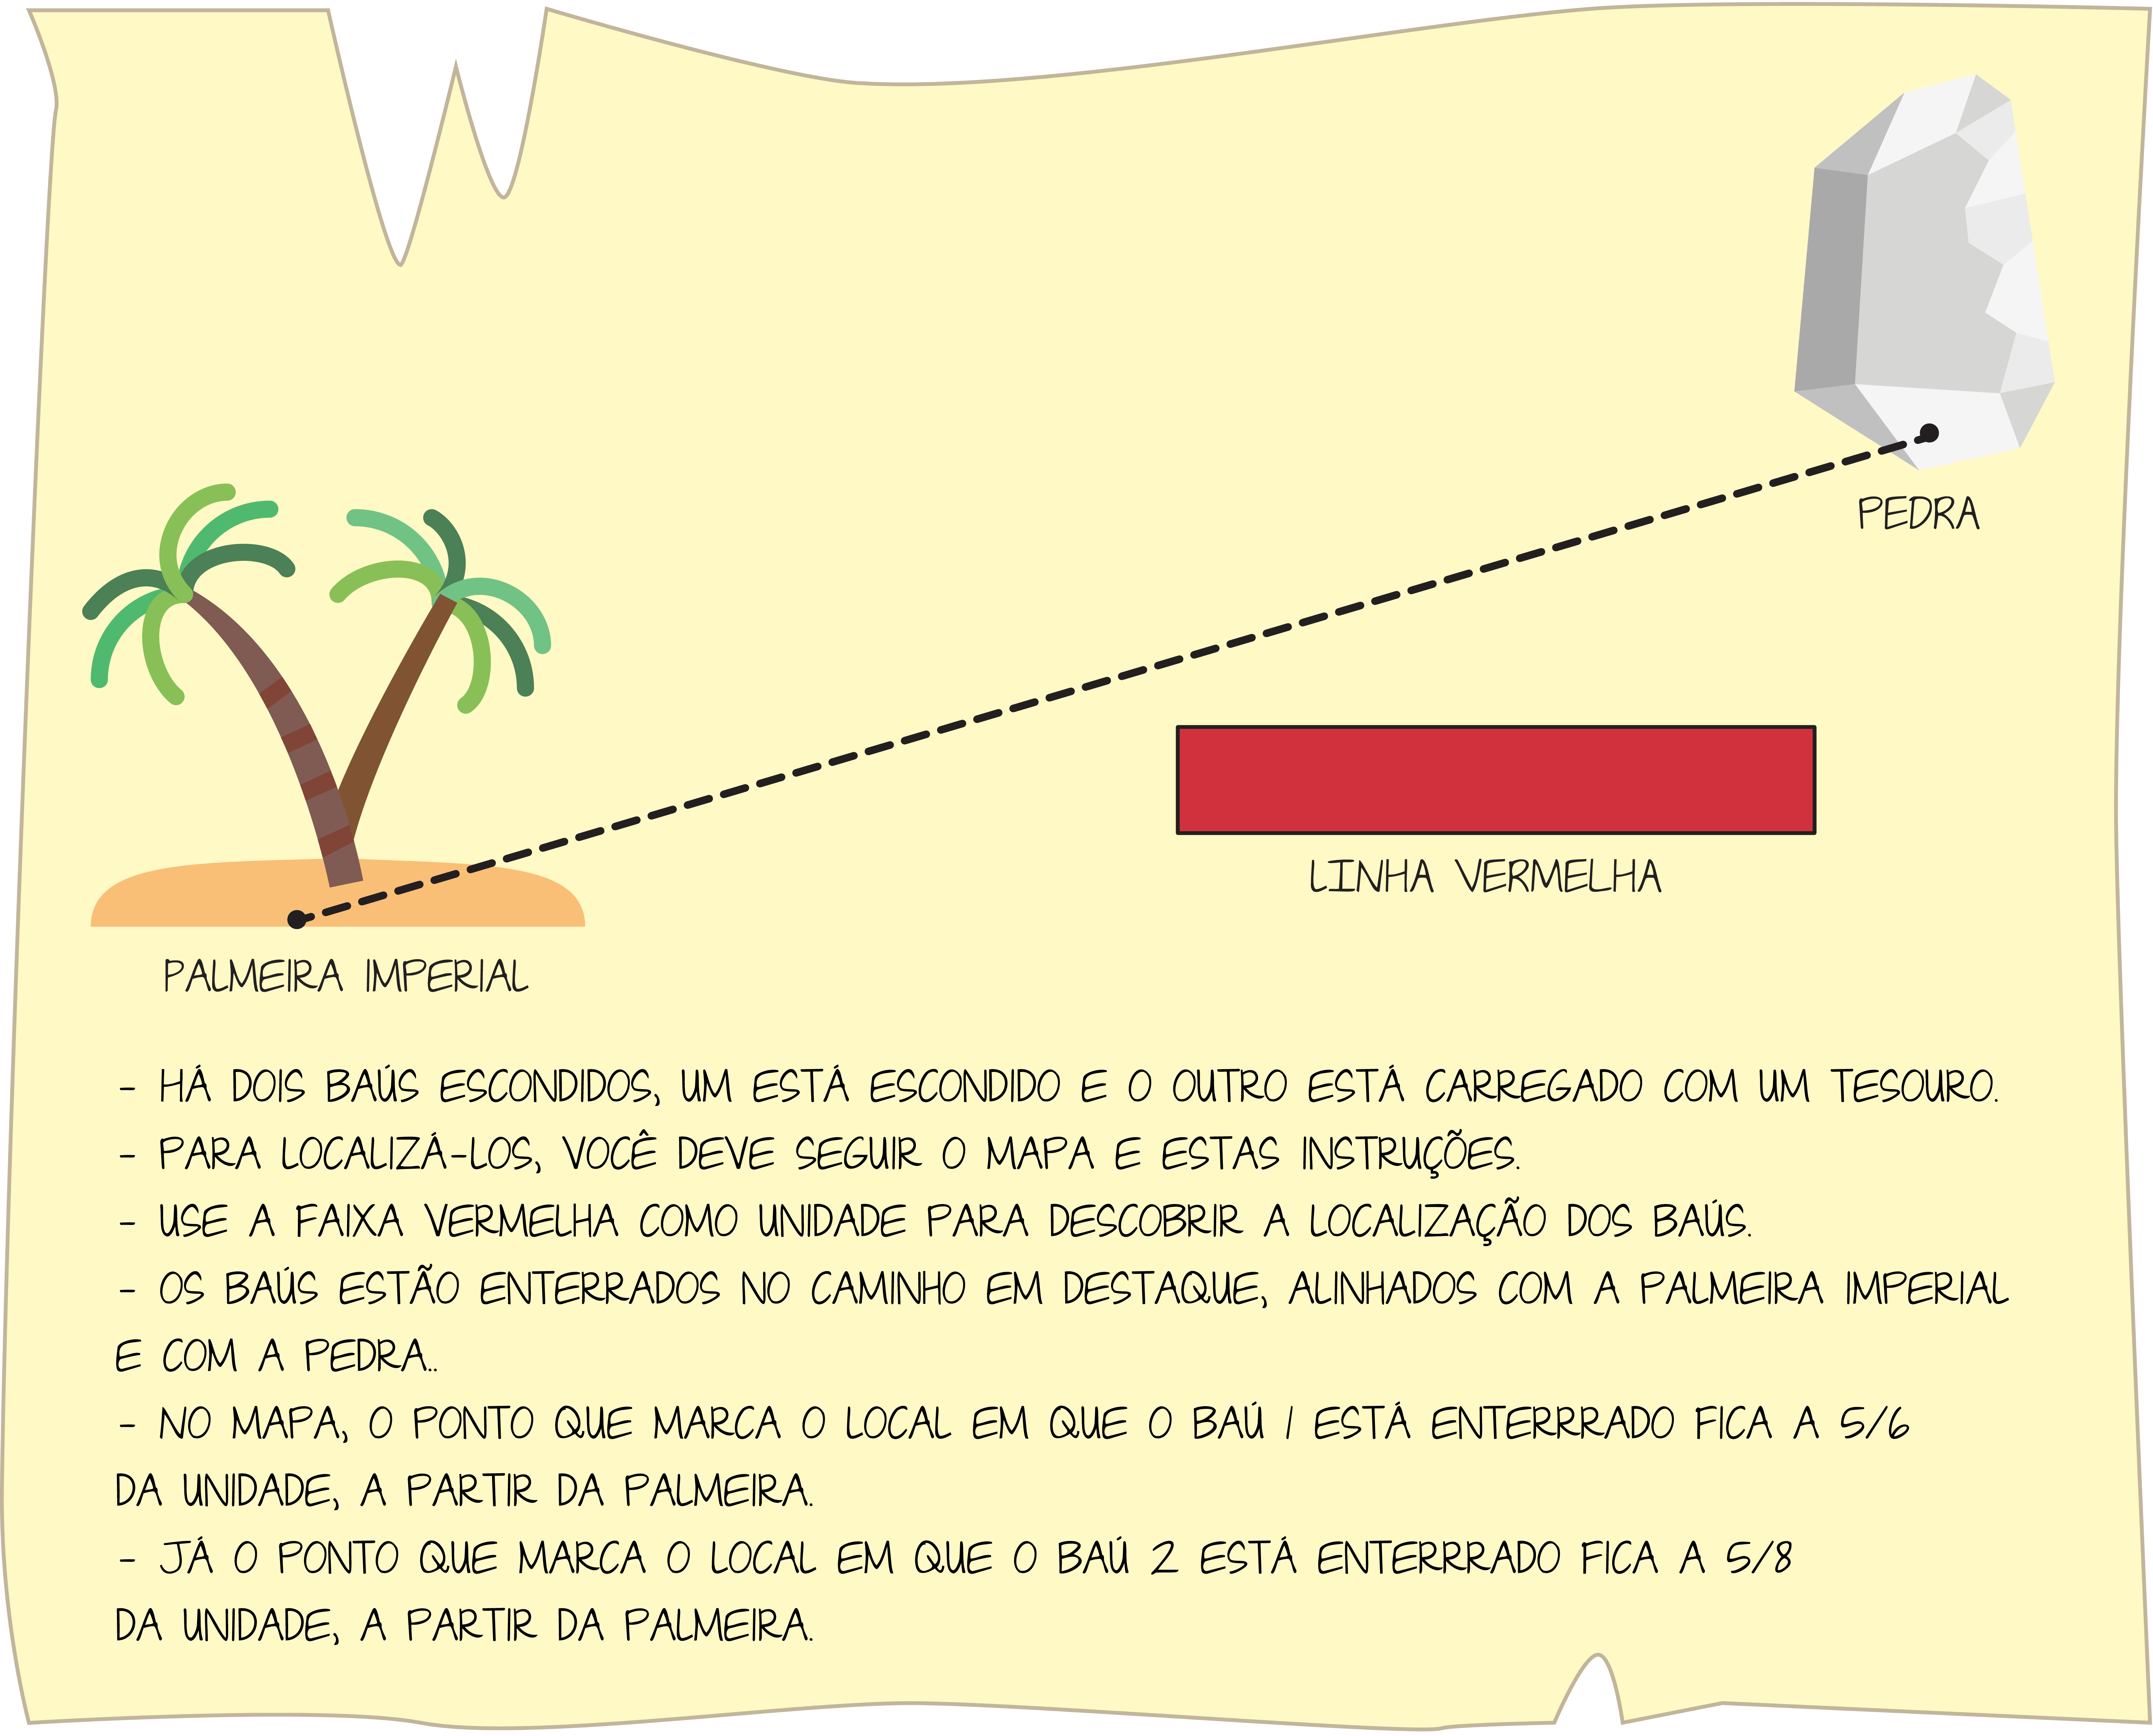
\includegraphics[width=\textwidth, keepaspectratio]{../figuras/licao03/ativ7_fig01.png}

\begin{enumerate}[a)]
 \item Marque, no mapa, as localizações dos baús e da chave.
 \item Qual o baú com o tesouro? Explique como chegou à sua conclusão.
\end{enumerate}
\end{atividade}

\begin{atividade}{}

Três amigos foram a uma pizzaria e cada um pediu uma pizza média, de três sabores diferentes: João comeu $\frac{3}{4}$ da pizza de calabresa, Maria comeu  $\frac{2}{4}$ da pizza de presunto e Miguel comeu $\frac{2}{5}$ da pizza de milho. Sabendo-se que todas as pizzas eram do mesmo tamanho, pergunta-se:
\begin{enumerate} [\quad a)] %s
  \item     Quem comeu mais pizza, João ou Maria? Explique.
  \item     E no caso de Maria e Miguel, quem comeu mais pizza? Explique.
  \item     Dos três amigos, quem comeu mais pizza? Explique.
  \item     Marque na reta numérica a seguir as frações correspondentes às porções de pizza que cada amigo comeu, e confira a sua resposta do item c).
\end{enumerate} %s

\begin{center}
 \begin{tikzpicture}[x=56.25mm,y=56.25mm]
\draw[->] (-0.2,0) -- (1.2,0) ; %edit here for the axis
\foreach \x in {0,1}{ \draw (\x,3pt) -- (\x,-3pt) node[below] {\x};}
\end{tikzpicture}
\end{center}
\end{atividade}

\begin{atividade}{}

A imagem a seguir ilustra uma tartaruga percorrendo um caminho em linha reta, do ponto de partida ao de chegada. Observe a posição da tartaruga na imagem e avalie se as afirmações a seguir estão corretas ou não. Em cada item, explique a sua avaliação por escrito.

\noindent
\includegraphics[width=\textwidth, keepaspectratio]{../figuras/licao03/ativ9_fig01b.png}

\begin{enumerate} [\quad a)] %s
  \item     A tartaruga percorreu mais do que a metade do percurso total.
  \item     A tartaruga percorreu mais do que     $\frac{3}{4}$     do percurso total.
  \item     A tartaruga percorreu mais do que     $\frac{3}{8}$     do percurso total.
  \item     A tartaruga percorreu menos do que     $\frac{3}{4}$     do percurso total.
  \item     A tartaruga percorreu menos do que     $\frac{2}{8}$     do percurso total.
  \item     A tartaruga percorreu menos do que     $\frac{2}{3}$     do percurso total.
  \item     A tartaruga percorreu     $\frac{3}{4}$     do percurso total.
  \item     A tartaruga percorreu pelo menos     $\frac{5}{8}$     do percurso total.
  \item     Para alcançar a chegada, a tartaruga precisa percorrer mais do que a metade do percurso total.
  \item     Para alcançar a chegada, a tartaruga precisa percorrer menos do que     $\frac{2}{3}$     do percurso total.
\end{enumerate} %s

\end{atividade}

\begin{atividade}{}

Na figura, há várias retas paralelas igualmente espaçadas e outra reta, destacada em vermelho, não paralela às demais. As retas paralelas marcam na reta destacada em vermelho pontos também igualmente espaçados. Um desses pontos corresponde ao zero e outro ao 1. Assim a reta vermelha pode ser considerada uma reta numérica.

\begin{center}
 \begin{tikzpicture}[x=56.25mm,y=56.25mm]

\begin{scope}
\clip (-.2,-.2) rectangle (.85,.85);

\begin{scope}[ rotate=45]
\foreach \x in {-1.1,-1,...,1.6}{
\draw[common] (\x,0) --+ (45:1);
\draw[common] (\x,0) --+ (45:-1);}

\draw[attention] (-0.2,0) -- (1.2,0) ; %edit here for the axis
\foreach \x in {0,1}{ \draw (\x,3pt) -- (\x,-3pt) node[below] {\x};}
\foreach \x in {0.1,.2,...,.9}{ \draw (\x,3pt) -- (\x,-3pt);}
\end{scope}
\end{scope}

\end{tikzpicture}
\end{center}

\begin{enumerate} [\quad a)] %s
  \item     Marque o ponto correspondente à fração $\frac{1}{2}$ na reta vermelha.
  \item     Escreva a fração correspondente a cada marcação na reta vermelha. Explique sua resposta.    \mbox{} \newline
  \end{enumerate}
  
  Na figura a seguir, há várias retas paralelas igualmente espaçadas e outra reta, destacada em azul, não paralela às anteriores. Observe que as retas paralelas marcam na reta destacada em azul pontos também igualmente espaçados. Dois desses pontos correspondem às frações $\frac{1}{2}$ e $\frac{3}{2}$, como ilustra a figura.

  \begin{center}
  \begin{tikzpicture}[x=56.25mm,y=56.25mm]

\begin{scope}
\clip (-.2,-.2) rectangle (.85,.85);

\begin{scope}[ rotate=45]
\foreach \x in {-1.1,-1,...,1.6}{
\draw[common] (\x,0) --+ (135:1);
\draw[common] (\x,0) --+ (135:-1);}

\draw[blue] (-0.2,0) -- (1.2,0) ; %edit here for the axis
\foreach \x in {0,0.1,.2,...,.9}{ \draw (\x,3pt) -- (\x,-3pt);}
\fill[common] (.2,0) circle (3pt) node[below, black] {$\frac{1}{2}$};
\fill[common] (.6,0) circle (3pt) node[below, black] {$\frac{3}{2}$};
\end{scope}
\end{scope}

\end{tikzpicture}
\end{center}

\begin{enumerate}[\quad a)]
  \item[c)]     Indique as marcações correspondentes ao zero e ao um na reta numérica.
  \item[d)]     Marque, nesta mesma reta numérica, as frações     $\frac{3}{4}$     e     $\frac{5}{4}$.
    \item[e)] Qual das marcações na reta azul representa a maior fração? Que fração é essa?

\end{enumerate} %s
\end{atividade}

\section{ORGANIZANDO AS IDEIAS }

Como se sabe, os números naturais podem ser representados por pontos em uma reta. Para isso, é preciso escolher um ponto para corresponder ao zero e outro para corresponder ao um. O segmento de extremos $0$ e $1$ é associado à unidade. Os pontos que corresponderão aos demais números naturais são obtidos a partir da unidade.

\begin{center}
 \begin{tikzpicture}[x=18mm,y=18mm]
\node[above] at (.5,3pt) {unidade};
\draw[->] (-0.5,0) -- (7.5,0) ; %edit here for the axis
\foreach \x in {0,1}{ \node[below] at (\x,-3pt) {\x};}
\draw[very thick, attention] (0,0) -- (1,0);
\foreach \x in {0,1}{ \fill[attention] (\x,0) circle (3pt);}
\end{tikzpicture}

\vspace{.2cm}


\begin{tikzpicture}[x=18mm,y=18mm]
\draw[->] (-0.5,0) -- (7.5,0) ; %reta 
\draw[very thick, attention] (0,0) -- (2,0);
\node[above] at (1,3pt) {2 unidades};
\draw (1,-3pt) -- (1,3pt);
\foreach \x in {0,1,2}{ \node[below] at (\x,-3pt) {\x}; }
%\fill[common] (1,0) circle (2pt);
\foreach \x in {0,2} \fill[attention] (\x,0) circle (3pt);
 % \fill[common] (0,0) circle (2pt);
\end{tikzpicture}

\vspace{.2cm}


\begin{tikzpicture}[x=18mm,y=18mm]

\draw[->] (-0.5,0) -- (7.5,0) ; %reta 
\draw[very thick, attention] (0,0) -- (7,0);
\node[above] at (3.5 , 3pt) {7 unidades};

\foreach \x in {1,2,3,4,5,6}{ \draw (\x,3pt) -- (\x,-3pt) node[below] {\x};}

\foreach \x in {0,7}
{
  \fill[attention] (\x,0) circle (3pt);
  \node[below] at (\x,-3pt) {\x};
}

 % \fill[common] (0,0) circle (2pt);
 % \fill[common] (1,0) circle (2pt);
  %\node[below] at (1,-3pt) {1};


\end{tikzpicture}
\end{center}

As frações também podem ser associadas a pontos na reta numérica. Para isso, é preciso dividir a unidade em partes iguais. Por exemplo, a divisão da unidade em $3$ partes iguais determina três terços. O ponto correspondente ao número $\frac{1}{3}$  é a extremidade do segmento que, a partir do $0$, identifica o primeiro terço da unidade. 

\begin{center}
  \begin{tikzpicture}[x=18mm,y=18mm]
\draw[->] (-0.5,0) -- (3.5,0) ; %reta anterior
\draw[very thick, attention] (0,0) -- (1,0);
\node[above] at (1/2,3pt) {unidade};
\foreach \x in {0,1,2,3}{ \draw (\x,3pt) -- (\x,-3pt) node[below] {\x};}

\draw (1/3,3pt) -- (1/3,-3pt);
\draw (2/3,3pt) -- (2/3,-3pt);

\foreach \x in {0,1}{ \fill[attention] (\x,0) circle (3pt);}
  \end{tikzpicture}
  \vspace{.2cm}

  %1/3 da unidade
  \begin{tikzpicture}[x=18mm,y=18mm]
\draw[->] (-0.5,0) -- (3.5,0) ; %reta anterior
\draw[very thick, attention] (0,0) -- (1/3,0);
\node[above] at (1/6,3pt) {$\frac{1}{3}$ da unidade};
\foreach \x in {0,1,...,3}{ \draw (\x,3pt) -- (\x,-3pt) node[below] {\x};}

\draw (2/3,3pt) -- (2/3,-3pt);
\node[below] at (1/3,-3pt) {$\dfrac{1}{3}$};
\foreach \x in {0,1/3}{ \fill[attention] (\x,0) circle (3pt);}
%\fill[common] (1/3,0) circle (3pt);
\end{tikzpicture}
\end{center}

A partir do ponto correspondente ao $\frac{1}{3}$, são marcados na reta numérica os pontos correspondentes a $\frac{2}{3}$, $\frac{3}{3}$, $\frac{4}{3}$, e assim por diante.

% 2/3 da unidade
\begin{center}
\begin{tikzpicture}[x=18mm,y=18mm]
\draw[->] (-0.5,0) -- (3.5,0) ; %reta anterior
\draw[very thick, attention] (0,0) -- (2/3,0);
\foreach \x in {0,1,2,3}{ \draw (\x,3pt) -- (\x,-3pt) node[below] {\x};}

%\draw (2/3,3pt) -- (2/3,-3pt);
\node[below] at (1/3,-3pt) {$\dfrac{1}{3}$};
\node[below] at (2/3,-3pt) {$\dfrac{2}{3}$};
\node[above] at (1/3,3pt) {$\frac{2}{3}$ da unidade};
\draw (1/3,-3pt) -- (1/3,3pt);
\foreach \x in {0,2/3}{ \fill[attention] (\x,0) circle (3pt);}
%\fill[common] (1/3,0) circle (2pt);
%\fill[common] (2/3,0) circle (3pt);
\end{tikzpicture}
\vspace{.2cm}

%3/3 da unidade
\begin{tikzpicture}[x=18mm,y=18mm]

\draw[->] (-0.5,0) -- (3.5,0) ; %reta anterior
\draw[very thick, attention] (0,0) -- (1,0);
\foreach \x in {0,2,3}{ \draw (\x,3pt) -- (\x,-3pt) node[below] {\x};}

\draw (2/3,3pt) -- (2/3,-3pt);
\node[below] at (1/3,-3pt) {$\dfrac{1}{3}$};
\node[below] at (2/3,-3pt) {$\dfrac{2}{3}$};
\node[below] at (1,-3pt) {$\dfrac{3}{3}$};
\node[above] at (1/2,3pt) {$\frac{3}{3}$ da unidade};
\draw (1/3,-3pt) -- (1/3,3pt);
\foreach \x in {0,3/3}{ \fill[attention] (\x,0) circle (3pt);}
%\fill[common] (1/3,0) circle (2pt);
%\fill[common] (2/3,0) circle (3pt);
\end{tikzpicture}
\vspace{.2cm}

%4/3 da unidade
\begin{tikzpicture}[x=18mm,y=18mm]

\draw[->] (-0.5,0) -- (3.5,0) ; %reta anterior
\draw[very thick, attention] (0,0) -- (4/3,0);
\foreach \x in {0,1,2,3}{ \draw (\x,3pt) -- (\x,-3pt) node[below] {\x};}

\draw (1/3,-3pt) -- (1/3,3pt);
\draw (2/3,3pt) -- (2/3,-3pt);
\node[below] at (1/3,-3pt) {$\dfrac{1}{3}$};
\node[below] at (2/3,-3pt) {$\dfrac{2}{3}$};
\node[below] at (4/3,-3pt) {$\dfrac{4}{3}$};

\node[above] at (2/3,3pt) {$\frac{4}{3}$ da unidade};

\foreach \x in {0,4/3}{ \fill[attention] (\x,0) circle (3pt);}
%\fill[common] (1/3,0) circle (2pt);
%\fill[common] (2/3,0) circle (3pt);
\end{tikzpicture}
\vspace{.2cm}

% todos os terços.
\begin{tikzpicture}[x=18mm,y=18mm]
\draw[->] (-0.5,0) -- (3.5,0) ; %reta anterior
%\draw[very thick, attention] (0,0) -- (1,0);
\foreach \x in {0,1,2,3}
{
  \node[above] at (\x,3pt) {\x};
}

%\foreach \x in {0,3,...,9}{ \fill[common] (\x/3,0) circle (3pt);
%\node[below] at (\x/3,0) {$\dfrac{\x}{3}$};}

\foreach \x in {0,1,2,3,4,5,6,7,8,9,10}
{
  \draw (\x/3,-3pt) -- (\x/3,3pt);
  \node[below] at (\x/3,-3pt) {$\dfrac{\x}{3}$};
}


\end{tikzpicture}
\end{center}

A representação dos números na reta numérica evidencia que algumas frações são números naturais. Por exemplo, $\frac{3}{3}$ é igual a 1. Portanto, $\frac{3}{3}$ de uma pizza é igual a 1 pizza e $\frac{3}{3}$ de uma barra de chocolate é igual a 1 barra de chocolate. 

\begin{center}
\begin{tabular}{ccc}
\parbox[100pt]{100pt}{\centering
\includegraphics[width=80pt, keepaspectratio]{../figuras/licao03/orgideias_fig_a.png}}  & \quad & 
\parbox[100pt]{100pt}{\centering\vfill
\includegraphics[width=95pt, keepaspectratio]{../figuras/licao03/orgideias_fig_b.png}
}
 \\
  \multicolumn{3}{c}
  {
\begin{tikzpicture}[x=18mm,y=18mm]
\draw[->] (-0.5,0) -- (3.5,0) ; %reta anterior
\draw[very thick, attention] (0,0) -- (1,0);

\foreach \x in {0,1,2,3}
{
  \node[below] at (\x/3,-3pt) {$\dfrac{\x}{3}$};
}

\foreach \x in {1,2}
{
  \draw (\x/3,-3pt) -- (\x/3,3pt);
}
\foreach \x in {2,3}
{
  \draw (\x,-3pt) -- (\x,3pt) node [above] {\x};
}

\foreach \x in {0,1}
{
  \fill [attention] (\x,0) circle (3pt);
  \node [above] at (\x,3pt) {\x}; % 0 e 1 inteiros.
}


\end{tikzpicture}
  }
\end{tabular}
\end{center}

Já $\frac{6}{3}$ é igual a $2$. Assim, $\frac{6}{3}$ de uma pizza é igual a $2$ pizzas e $\frac{6}{3}$ de uma barra de chocolate é igual a $2$ barras de chocolate.

\begin{center}
\begin{tabular}{lcc}
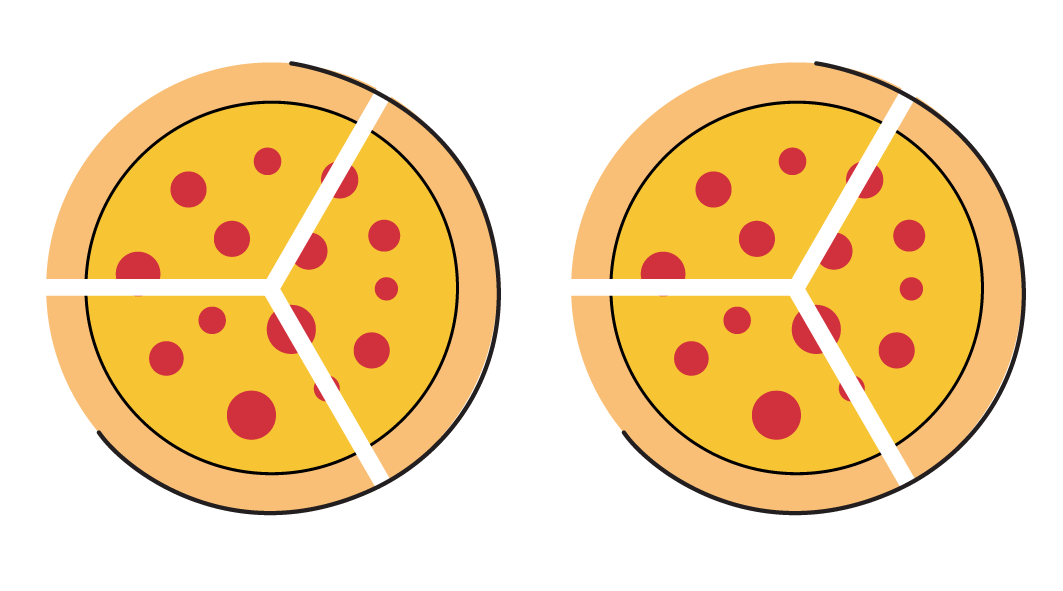
\includegraphics[width=180pt, keepaspectratio]{../figuras/licao03/orgideias_fig_a_2.png} &\quad &

\includegraphics[width=100pt, keepaspectratio]{../figuras/licao03/orgideias_fig_b_2.png} \\
  \multicolumn{3}{c}
  {
\begin{tikzpicture}[x=18mm,y=18mm]
\draw[->] (-0.5,0) -- (4.5,0) ; %reta anterior
\draw[very thick, attention] (0,0) -- (2,0);

\foreach \x in {0,...,6}
{
  \node[below] at (\x/3,-3pt) {$\dfrac{\x}{3}$};
}

\foreach \x in {1,2,3,4,5}
{
  \draw (\x/3,-3pt) -- (\x/3,3pt);
}


\foreach \x in {0,2}
{
  \fill [attention] (\x,0) circle (3pt);
  \node [above] at (\x,3pt) {\x}; % 0 e 2 inteiros.
}

\foreach \x in {1,3,4}
{
  \node [above] at (\x,3pt) {\x};
}

\draw (3,-3pt) -- (3,3pt);
\draw (4,-3pt) -- (4,3pt);
\end{tikzpicture}
  }
\end{tabular}
\end{center}


E $\frac{12}{3}$, é igual a que número natural? $\frac{12}{3}=$ {\Large $\square$}

Para identificar na reta numérica os pontos correspondentes às frações $\frac{1}{4}$, $\frac{2}{4}$, $\frac{3}{4}$, $\frac{4}{4}$, $\frac{5}{4}$, $\frac{6}{4}$, e assim por diante, o processo é o mesmo:

\begin{center}
 \begin{tikzpicture}[x=27mm,y=18mm]
\draw[->] (-0.5,0) -- (4.75,0) ; %reta anterior
\foreach \x in {0,1,...,4}{ \draw (\x,3pt) -- (\x,-3pt);
\node[above] at (\x,3pt) {\x};}

\foreach \x in {0,1,...,18}
{
  \node[below] at (\x/4,-3pt) {$\dfrac{\x}{4}$};
}

\foreach \x in {1,2,3,5,6,7,9,10,11,13,14,15,17,18}
{
  \draw (\x/4,-2pt) -- (\x/4,2pt);
}

\end{tikzpicture}
\end{center}

Na reta numérica a seguir estão destacados alguns pontos e as frações correspondentes a eles. Observe e complete as frações em destaque escrevendo seus numeradores.

\begin{center}
 \begin{tikzpicture}[x=18mm,y=18mm]
\draw[->] (-0.5,0) -- (3.7,0) ; %reta anterior
%\draw[very thick, attention] (0,0) -- (1,0);
\foreach \x in {0,1,...,20}{ \draw (\x/6,2pt) -- (\x/6,-2pt);}
\foreach \x in {0,1,...,3}{ \draw (\x,3pt) -- (\x,-3pt) node[below] {\x};}

\foreach \x in {4,15,20}{ \fill[attention] (\x/6,0) circle (3pt);
\node[below] at (\x/6,-3pt) {$\dfrac{\square}{6}$};}

\foreach \x in {2,9}{ \node[below] at (\x/6,-3pt) {$\dfrac{\x}{6}$};}

\end{tikzpicture}
\end{center}

\noindent{\bf A ordem na reta numérica}

\noindent Como você pode perceber, os números são organizados na reta numérica em ordem crescente no sentido que vai do zero para o um. As marcações do 0 e do 1 informam a ordem crescente. 

\begin{center}
 \begin{tikzpicture}[x=18mm,y=18mm]
\node[above] at (3,3pt) {Ordem crescente};
\draw[->] (-0.5,0) -- (3.5,0) ; %edit here for the axis
\foreach \x in {0,1}{\node[below] at (\x,-3pt) {\x};}
%\draw[very thick, attention] (0,0) -- (1,0);
\foreach \x in {0,1}{ \fill[attention] (\x,0) circle (3pt);}
\end{tikzpicture}
\end{center}
\begin{minipage}[l]{.45\linewidth}

 \setlength{\parindent}{18pt} A organização dos números na reta numérica permite comparar dois números apenas observando a sua posição na reta. Por exemplo, observando a ordem crescente, como 5 está adiante do 3, o número 5 é maior do que o número 3, ou, em símbolos matemáticos, $5 > 3$. O mesmo vale para as frações. Como $\frac{3}{2}$ está antes de $\frac{7}{3}$, sabe-se que $\frac{3}{2}$ é menor do que $\frac{7}{3}$, ou, em símbolos matemáticos $\frac{3}{2} < \frac{7}{3}$. É possível perceber que $\frac{7}{3} < 3$. 

\begin{center}
 \begin{tikzpicture}[x=18mm,y=18mm, rotate=20]
\draw[->] (-0.5,0) -- (3.5,0) ; %edit here for the axis

\foreach \x in {0,1,2}
{
  \draw (\x,3pt) -- (\x,-3pt);
  \node[below] at (\x,-3pt) {\x};
}

\foreach \x in {3/2,7/3,3}
{
  \fill [attention] (\x,0) circle (3pt);
}

\node [below] at (3/2,-3pt) {$\frac{3}{2}$};
\node [below] at (7/3,-3pt) {$\frac{7}{3}$};
\node [below] at (3,-3pt) {$3$};

\end{tikzpicture}
\end{center}

\end{minipage}\hfill
\begin{minipage}[r]{.5\linewidth}
\begin{caixinha}{}{}
O símbolo ''$<$'' é usado para dizer ''é menor do que'' e o símbolo ''$>$'' significa ''é maior do que''. Assim, por exemplo, a frase ''oito é menor do que quinze'' pode ser expressa de modo mais resumido como \mbox{$8<15$}. Já a expressão \mbox{$\frac{3}{2}  > \frac{1}{2}$} quer dizer que ''três meios é maior do que um meio''.

% \begin{center}
%   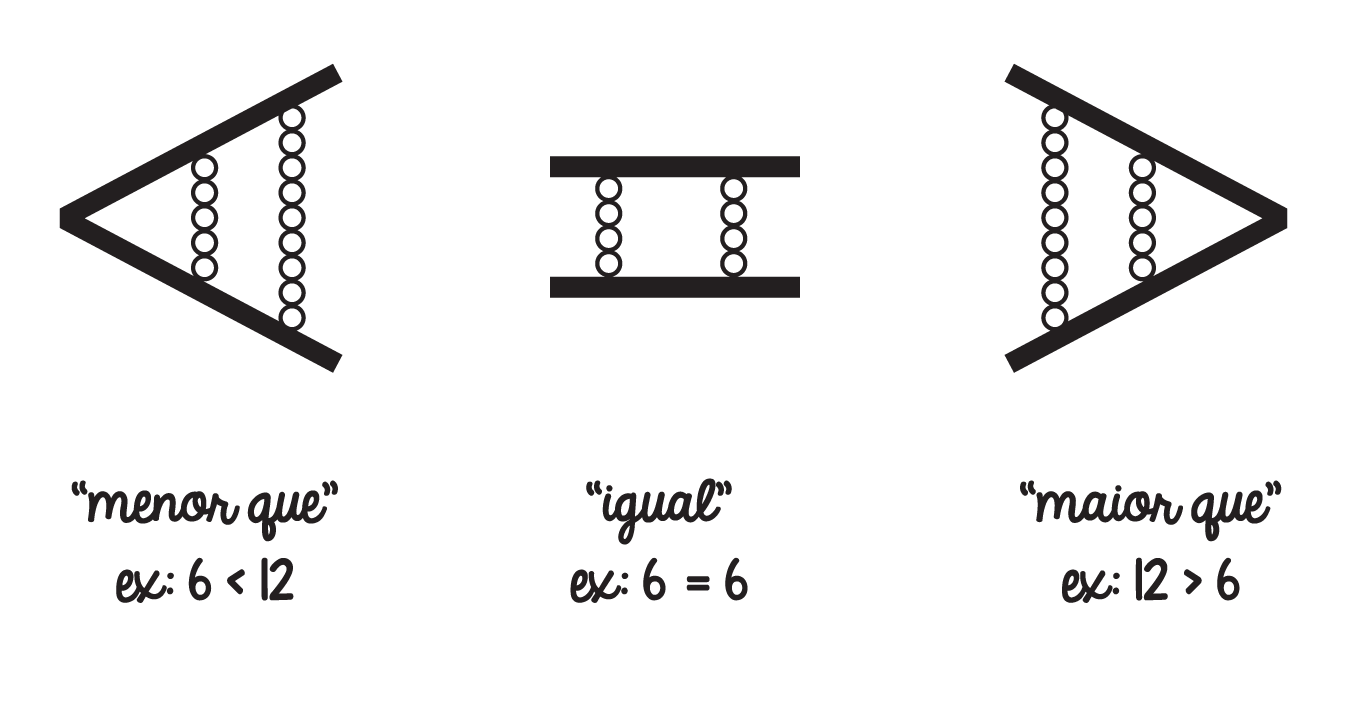
\includegraphics[width=150pt, keepaspectratio]{../figuras/licao03/orgideias_fig05.png}
% \end{center}

\setlength{\parindent}{-30pt} \begin{tikzpicture}[scale=1.3]
    \node at (0,0) {\scalebox{5.2}{$<$}};
    \node at (20,0) {\scalebox{5.2}{$=$}};
    \node at (40,0) {\scalebox{5.2}{$>$}};
    \begin{scope}[xshift=4]
      \def\r{1.4pt}
      \foreach \x in {-2,-1,0,1,2}
      {
        \fill[common, opacity=.5] (0,2*\x*\r) circle (\r);
      }
      \foreach \x in {-4,-3,-2,-1,0,1,2,3,4}
      {
        \fill[common, opacity=.5] (4,2*\x*\r) circle (\r);
      }
    \end{scope}
  \def\r{1.2pt}
      \foreach \x in {-1,0,1}
      {
        \fill[common, opacity=.5] (16,2*\x*\r +3.3) circle (\r);
        \fill[common, opacity=.5] (24,2*\x*\r + +3.3) circle (\r);
      }
     \begin{scope}[xshift=109.8, rotate=180]
      \def\r{1.4pt}
      \foreach \x in {-2,-1,0,1,2}
      {
        \fill[common, opacity=.5] (0,2*\x*\r) circle (\r);
      }
      \foreach \x in {-4,-3,-2,-1,0,1,2,3,4}
      {
        \fill[common, opacity=.5] (4,2*\x*\r) circle (\r);
      }
    \end{scope}

    \node [text width=2.8cm,align=center] at (0,-15) {{\footnotesize ''é menor do que''\\ $5<9$}};
    \node [text width=3cm,align=center] at (20,-13.5) {{\footnotesize ''é igual a''\\ $3=3$}};
    \node [text width=2.7cm,align=center] at (39,-15) {{\footnotesize ''é maior do que''\\ $9>5$}};
\end{tikzpicture}

\end{caixinha}

\end{minipage}


 Mesmo sem saber que números são $a$ e $b$, observando as suas representações na reta numérica, podemos concluir que $a < b$.

\begin{center}
 \begin{tikzpicture}[x=18mm,y=18mm]
\draw[->] (-0.5,0) -- (3.5,0) ; %edit here for the axis
\foreach \x in {0,1}{\node[below] at (\x,-3pt) {$\x$};}
%\draw[very thick, attention] (0,0) -- (1,0);
\foreach \x in {0,1}
{
\draw (\x,3pt) -- (\x,-3pt);
}
\foreach \x/\c/\n in {1.2/attention/a,2/attention/b}
{
  \fill [\c] (\x,0) circle (3pt);
  \node [below] at (\x,-3pt) {$\n$};
}

\end{tikzpicture}
\end{center}

E neste caso, qual é o menor número, $c$ ou $d$?

\begin{center}
 \begin{tikzpicture}[x=18mm,y=18mm, rotate=-15]
\draw[->] (-0.5,0) -- (3.5,0) ; %edit here for the axis
\foreach \x in {0,1}{\node[below] at (\x,-3pt) {$\x$};}
%\draw[very thick, attention] (0,0) -- (1,0);
\foreach \x in {0,1}
{
\draw (\x,3pt) -- (\x,-3pt);
}
\foreach \x/\c/\n in {0.8/attention/d,1.6/attention/c}
{
  \fill [\c] (\x,0) circle (3pt);
  \node [below] at (\x,-3pt) {$\n$};
}

\end{tikzpicture}
\end{center}

O número $d$ é menor que $c$ porque, observando a ordem crescente, $d$ está antes de $c$. É possível concluir ainda que $d$ é um número menor do que 1 e $c$ um número maior do que 1. 

\section{MÃO NA MASSA }

\begin{atividade}{}

{\bf Jogo: varal dos números}

O varal de números está disposto na sala de aula, nele já estão posicionados os números $0$ (zero) e $1$ (um), como na figura. Nos cartões preparados para a atividade estão os números: \\
$0$, $1$, $2$, $3$, $\frac{1}{2}$, $\frac{2}{2}$, $\frac{3}{2}$, $\frac{4}{2}$, $\frac{5}{2}$, $\frac{6}{2}$,
$\frac{1}{3}$, $\frac{2}{3}$, $\frac{3}{3}$, $\frac{4}{3}$, $\frac{7}{3}$, $\frac{9}{3}$,
$\frac{1}{4}$, $\frac{2}{4}$, $\frac{3}{4}$, $\frac{4}{4}$, $\frac{5}{4}$, $\frac{6}{4}$, $\frac{8}{4}$, $\frac{10}{4}$, $\frac{11}{4}$, $\frac{12}{4}$,
$\frac{1}{5}$, $\frac{3}{5}$, $\frac{4}{5}$, $\frac{6}{5}$, $\frac{7}{5}$, $\frac{10}{5}$,
$\frac{1}{10}$.

\begin{center}
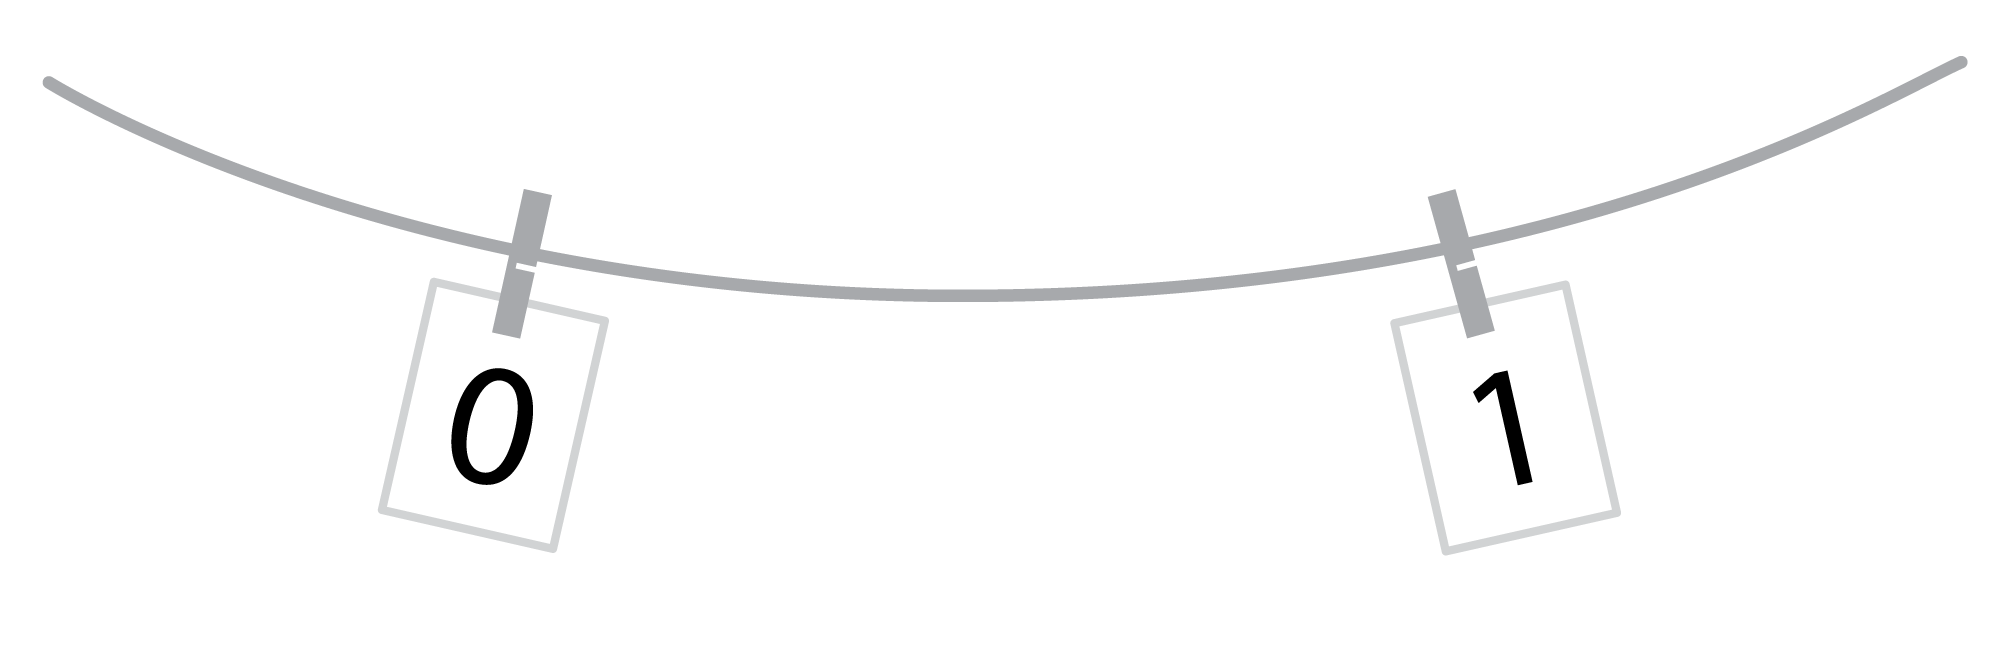
\includegraphics[width=300pt, keepaspectratio]{../figuras/licao03/ativ11_fig01.png}
\end{center}


O jogo consiste em fixar cartões numerados em varal, reproduzindo uma reta numérica. As regras serão apresentadas pelo seu professor ou professora. Discuta com seus colegas a posição correta de fixação de cada um dos cartões numerados no varal.

Ao final do jogo, reproduza a forma como os cartões foram posicionados no varal na reta numérica a seguir. Aproveite as marcações já existentes.

\begin{center}
\begin{tikzpicture}[x=34mm,y=34mm]
\draw[->] (-0.1,0) -- (4,0) ; %reta anterior
\foreach \x in {0,.1,...,3.9}{ \draw (\x,3pt) -- (\x,-3pt);}
\end{tikzpicture}
\end{center}
\end{atividade}

\begin{atividade}{}

Na reta numérica já estão marcados os números 0, 1 e $\frac{1}{2}$. Marque $\frac{3}{2}$, $\frac{3}{4}$, $\frac{5}{4}$, $\frac{8}{4}$, $\frac{10}{4}$, $\frac{1}{8}$, $\frac{7}{8}$, $\frac{10}{8}$ e 2.

\begin{center}
 \begin{tikzpicture}[x=5mm,y=5mm]
	\draw[->]  (-0.5,0) -- (26,0);
	\draw  (0,-3pt) -- (0,3pt);
	\draw  (1.25,-3pt) -- (1.25,3pt);
	\draw  (2.5,-3pt) -- (2.5,3pt);
	\draw  (3.75,-3pt) -- (3.75,3pt);
	\draw  (5,-3pt) -- (5,3pt);
	\draw  (6.25,-3pt) -- (6.25,3pt);
	\draw  (7.5,-3pt) -- (7.5,3pt);
	\draw  (8.75,-3pt) -- (8.75,3pt);
	\draw  (10,-3pt) -- (10,3pt);
	\draw  (11.25,-3pt) -- (11.25,3pt);
	\draw  (12.5,-3pt) -- (12.5,3pt);
	\draw  (13.75,-3pt) -- (13.75,3pt);
	\draw  (15,-3pt) -- (15,3pt);
	\draw  (16.25,-3pt) -- (16.25,3pt);
	\draw  (17.5,-3pt) -- (17.5,3pt);
	\draw  (18.75,-3pt) -- (18.75,3pt);
	\draw  (20,-3pt) -- (20,3pt);
	\draw  (21.25,-3pt) -- (21.25,3pt);
	\draw  (22.5,-3pt) -- (22.5,3pt);
	\draw  (23.75,-3pt) -- (23.75,3pt);
	\draw  (25,-3pt) -- (25,3pt);

	\node[below] at (0,0) {0};
	\node[below] at (5,0) {$\frac{1}{2}$};
	\node[below] at (10,0)  {1};

\end{tikzpicture}
\end{center}
\end{atividade}
\begin{atividade}[label=chap3-ativ13]{}
\phantomsection

Associe, como no exemplo, cada  fração à sua representação na reta numérica.

\noindent\begin{tabular}{m{.09\textwidth}m{.08\textwidth}m{.08\textwidth}m{.08\textwidth}m{.08\textwidth}m{.08\textwidth}m{0.08\textwidth}m{.08\textwidth}m{0.08\textwidth}}
(A) $\frac{1}{2}$ & (B) $\frac{1}{3}$ &  (C) $\frac{1}{4}$  & (D) $\frac{1}{5}$ & (E) $\frac{1}{6}$  & (F) $\frac{1}{7}$  & (G) $\frac{1}{8}$  & (H) $\frac{1}{9}$  & (I) $\frac{1}{10}$
\end{tabular}

\begin{center}
\begin{longtable}{m{.2\textwidth}m{.5\textwidth}}

\centering \begin{tikzpicture}
 \draw (0,0) -- (20,0);
\end{tikzpicture}
 &
\parbox[t][1cm][c]{8cm}{
\begin{tikzpicture}[x=50mm,y=50mm]
\draw[->] (-0.3,0) -- (1.3,0) ; %reta anterior
\foreach \x in {0,.1,1}{ \draw (\x,3pt) -- (\x,-3pt);}
 \node[below] at (0,0) {0};
 \node[below] at (1,0) {1};
 \fill[common] (.1,0) circle (3pt);
\end{tikzpicture}}
\\

 \centering \begin{tikzpicture}
 \draw (0,0) -- (20,0);
 \node[above] at (10,0){(A)};
\end{tikzpicture}
 &
\parbox[t][1cm][c]{8cm}{
\begin{tikzpicture}[x=50mm,y=50mm]
\draw[->] (-0.3,0) -- (1.3,0) ; %reta anterior
\foreach \x in {0,1}{ \draw (\x,3pt) -- (\x,-3pt);}
 \node[below] at (0,0) {0};
 \node[below] at (1,0) {1};
 \fill[common] (.5,0) circle (3pt);
\end{tikzpicture}
}\\

\centering \begin{tikzpicture}
 \draw (0,0) -- (20,0);
\end{tikzpicture}
  &
\parbox[t][1cm][c]{8cm}{
\begin{tikzpicture}[x=50mm,y=50mm]
\draw[->] (-0.3,0) -- (1.3,0) ; %reta anterior
\foreach \x in {0,1}{ \draw (\x,3pt) -- (\x,-3pt);}
 \node[below] at (0,0) {0};
 \node[below] at (1,0) {1};
 \fill[common] (1/3,0) circle (3pt);
\end{tikzpicture}
}\\

\centering \begin{tikzpicture}
 \draw (0,0) -- (20,0);
\end{tikzpicture}
 &
\parbox[t][1cm][c]{8cm}{
\begin{tikzpicture}[x=50mm,y=50mm]
\draw[->] (-0.3,0) -- (1.3,0) ; %reta anterior
\foreach \x in {0,1}{ \draw (\x,3pt) -- (\x,-3pt);}
 \node[below] at (0,0) {0};
 \node[below] at (1,0) {1};
 \fill[common] (1/9,0) circle (3pt);
\end{tikzpicture}
}\\

\centering \begin{tikzpicture}
 \draw (0,0) -- (20,0);
\end{tikzpicture}
 &
\parbox[t][1cm][c]{8cm}{
\begin{tikzpicture}[x=50mm,y=50mm]
\draw[->] (-0.3,0) -- (1.3,0) ; %reta anterior
\foreach \x in {0,1}{ \draw (\x,3pt) -- (\x,-3pt);}
 \node[below] at (0,0) {0};
 \node[below] at (1,0) {1};
 \fill[common] (1/7,0) circle (3pt);
\end{tikzpicture}
}\\

\centering \begin{tikzpicture}
 \draw (0,0) -- (20,0);
\end{tikzpicture}
 &
\parbox[t][1cm][c]{8cm}{
\begin{tikzpicture}[x=50mm,y=50mm]
\draw[->] (-0.3,0) -- (1.3,0) ; %reta anterior
\foreach \x in {0,1}{ \draw (\x,3pt) -- (\x,-3pt);}
 \node[below] at (0,0) {0};
 \node[below] at (1,0) {1};
 \fill[common] (.25,0) circle (3pt);
\end{tikzpicture}
}\\

\centering \begin{tikzpicture}
 \draw (0,0) -- (20,0);
\end{tikzpicture}
 &
\parbox[t][1cm][c]{8cm}{
\begin{tikzpicture}[x=50mm,y=50mm]
\draw[->] (-0.3,0) -- (1.3,0) ; %reta anterior
\foreach \x in {0,1}{ \draw (\x,3pt) -- (\x,-3pt);}
 \node[below] at (0,0) {0};
 \node[below] at (1,0) {1};
 \fill[common] (1/6,0) circle (3pt);
\end{tikzpicture}
}\\

\centering \begin{tikzpicture}
 \draw (0,0) -- (20,0);
\end{tikzpicture}
&
\parbox[t][1cm][c]{8cm}{
\begin{tikzpicture}[x=50mm,y=50mm]
\draw[->] (-0.3,0) -- (1.3,0) ; %reta anterior
\foreach \x in {0,1}{ \draw (\x,3pt) -- (\x,-3pt);}
 \node[below] at (0,0) {0};
 \node[below] at (1,0) {1};
 \fill[common] (1/5,0) circle (3pt);
\end{tikzpicture}
}\\

\centering \begin{tikzpicture}
 \draw (0,0) -- (20,0);
\end{tikzpicture}
&
\parbox[t][1cm][c]{8cm}{
\begin{tikzpicture}[x=50mm,y=50mm]
\draw[->] (-0.3,0) -- (1.3,0) ; %reta anterior
\foreach \x in {0,1}{ \draw (\x,3pt) -- (\x,-3pt);}
 \node[below] at (0,0) {0};
 \node[below] at (1,0) {1};
 \fill[common] (1/8,0) circle (3pt);
\end{tikzpicture}
}\\

\end{longtable}
\end{center}
\end{atividade}
\begin{atividade}{}

Complete as sentenças a seguir com os sinais $>$ (maior) ou $<$ (menor) de modo a torná-las verdadeiras.
\begin{center}
\begin{tabular}{ccccccccc}
 a)  &   $\dfrac{1}{2}$    & \parbox[t][.6cm]{2cm}{ }\;\,{\huge $\square$} \quad      &  $\dfrac{1}{5}$ & \quad\quad\quad\quad\quad\quad\quad   &e)  &  $\dfrac{1}{35}$   & \,{\huge $\square$}\quad      &  $\dfrac{1}{43}$\\
 b)  &  $\dfrac{1}{4}$    & \parbox[t][.6cm]{2cm}{ }{\huge $\square$}      &  $\dfrac{1}{3}$   & & f)  &  $\dfrac{1}{99}$   &  {\huge $\square$}     &  $\dfrac{1}{100}$  \\
 c)  &  $\dfrac{1}{10}$   &  \parbox[t][.6cm]{2cm}{ }{\huge $\square$}     &  $\dfrac{1}{20}$  & & g)  &  $\dfrac{1}{5}$    &  {\huge $\square$}     &  $\dfrac{1}{50}$  \\
 d)  &  $\dfrac{1}{12}$   & \parbox[t][.6cm]{2cm}{ }{\huge $\square$}      &  $\dfrac{1}{2}$   & & h)  &  $\dfrac{1}{100}$  & {\huge $\square$}      &  $\dfrac{1}{10}$  \\
 \end{tabular}
 \end{center}
\end{atividade}

\begin{atividade}{}

Na reta numérica a seguir estão identificados os pontos correspondentes aos números 0, 1 e $\frac{1}{2}$. Os demais pontos correspondem aos números   apresentados a seguir. Associe cada fração ao ponto correspondente na reta numérica.

\begin{center}
\begin{tikzpicture}[x=.3cm,y=.3cm,]
	\draw[->] (-2,0) -- (47,0);

	\fill[common] (0,0) circle (3 pt);		%0
	\fill[common] (10,0) circle (3 pt);
	\fill[common] (15,0) circle (3 pt);
	\fill[common] (20,0) circle (3 pt);
	\fill[common] (25,0) circle (3 pt);
	\fill[common] (30,0) circle (3 pt);
	\fill[common] (32,0) circle (3 pt);
	\fill[common] (36,0) circle (3 pt);
	\fill[common] (40,0) circle (3 pt);
	\fill[common] (44,0) circle (3 pt);
	\fill[common] (45,0) circle (3 pt);

		\node[below]  at (0,-1) {0};			%0
		\node[below]  at (20,-1) {$\frac{1}{2}$};	%1/2
		\node[below]  at (40,-1) {1};			%1

	 	     \tikzstyle{gray_block} = [draw,outer sep=3,inner sep=3,minimum size=1,line width=1, very thick, draw=black!55, top color=white,bottom color=black!20]
	\node [gray_block] at (10.5,5) {$\frac{1}{4}$};
  	\node [gray_block] at (14.5,5) {$\frac{3}{4}$};
	\node [gray_block] at (18.5,5) {$\frac{4}{5}$};
	\node [gray_block] at (22.5,5) {$\frac{3}{8}$};
	\node [gray_block] at (26.5,5) {$\frac{5}{8}$};
	\node [gray_block] at (30.5,5) {$\frac{9}{8}$};
	\node [gray_block] at (35,5) {$\frac{9}{10}$};
	\node [gray_block] at (40,5) {$\frac{11}{10}$};
\end{tikzpicture}
\end{center}
\end{atividade}

\begin{atividade}{}


Complete as sentenças a seguir com os sinais $>$ (maior), $<$ (menor) ou $=$ (igual) de modo a torná-las verdadeiras.

\begin{center}
\begin{tabular}{lccccccccccccc}
 a)  &  $\dfrac{3}{6}$     &{\huge $\square$}  &  $\dfrac{5}{6}$   & \parbox[t][.6cm]{2cm}{ } \quad \quad\quad  & f)  &  $\dfrac{1}{2}$     & {\huge $\square$} &  $\dfrac{1}{3}$    & \quad \quad\quad  & m)  &  $\dfrac{3}{2}$     & {\huge $\square$} &  $\dfrac{2}{5}$    \\
 b)  &  $\dfrac{5}{9}$     &{\huge $\square$}&  $\dfrac{4}{9}$   & \parbox[t][.6cm]{2cm}{ }    & g)  &  $\dfrac{1}{7}$     &{\huge $\square$} &  $\dfrac{1}{6}$    &   & n)  &  $\dfrac{3}{4}$     &{\huge $\square$} &  $\dfrac{6}{5}$    \\
 c)  &  $\dfrac{27}{10}$    &{\huge $\square$} &  $\dfrac{29}{10}$   & \parbox[t][.6cm]{2cm}{ }   & h)  &  $\dfrac{2}{5}$     &{\huge $\square$}&  $\dfrac{2}{7}$    &   & o)  &  $\dfrac{7}{8}$     &{\huge $\square$} &  $\dfrac{10}{9}$   \\
 d)  &  $\dfrac{3}{12}$    &{\huge $\square$}&  $\dfrac{9}{12}$   & \parbox[t][.6cm]{2cm}{ }   & i)  &  $\dfrac{4}{5}$     &{\huge $\square$}&  $\dfrac{4}{3}$    &   & p)  &  $\dfrac{6}{5}$     &{\huge $\square$}&  $\dfrac{12}{9}$   \\
 e)  &  $\dfrac{139}{100}$  &{\huge $\square$}&  $\dfrac{125}{100}$ & \parbox[t][.6cm]{2cm}{ }   & j)  &  $\dfrac{12}{15}$   &{\huge $\square$}&  $\dfrac{12}{7}$   &   & q)  &  $\dfrac{4}{5}$     &{\huge $\square$}&  $\dfrac{5}{4}$    \\
     &&                     &    &                  \parbox[t][.6cm]{2cm}{ }    &  l)  &  $\dfrac{22}{80}$   &{\huge $\square$}&  $\dfrac{22}{90}$  &   & r)  &  $\dfrac{35}{40}$   &{\huge $\square$}&  $\dfrac{30}{25}$  \\
     &&                      &    &                    &      &  \parbox[t][.6cm]{2cm}{ }                    &   &                   &   &  s)  &  $\dfrac{99}{100}$  &{\huge $\square$}&  $\dfrac{3}{2}$    \\
\end{tabular}
 \end{center}
\end{atividade}
\section{QUEBRANDO A CUCA }


\begin{atividade}{}

  Você recebeu uma folha com 11 retângulos coloridos de mesmo tamanho. Cada retângulo está dividido em uma determinada quantidade de partes iguais.
  
\begin{enumerate}[a)]
\item Complete os retângulos escrevendo em cada uma das partes a fração correspondente, como no exemplo: o retângulo laranja está dividido em duas partes iguais, então cada parte é $\frac{1}{2}$.

\begin{center}
\begin{tikzpicture}[scale=.5, rotate=90]
\draw[fill=gray] (0,0) rectangle (60,12);


\begin{scope}[yshift=-40pt]
\draw[fill=light] (0,0) rectangle (60,12);
\draw (30,0) -- (30,12);
\node at (15,6) {{\small $\frac{1}{2}$}};
\node at (45,6) {{\small $\frac{1}{2}$}};


   \begin{scope}[yshift=-40pt]
\draw[fill=pink] (0,0) rectangle (60,12);
\foreach \x in {1,2} \draw (\x*60/3,0) -- (\x*60/3,12);


      \begin{scope}[yshift=-40pt]
\draw[fill=special] (0,0) rectangle (60,12);
\foreach \x in {1,2,3} \draw (\x*60/4,0) -- (\x*60/4,12);


   \begin{scope}[yshift=-40pt]
\draw[fill=attention] (0,0) rectangle (60,12);
\foreach \x in {1,...,4} \draw (\x*60/5,0) -- (\x*60/5,12);


   \begin{scope}[yshift=-40pt]
\draw[fill=common] (0,0) rectangle (60,12);
\foreach \x in {1,...,5} \draw (\x*60/6,0) -- (\x*60/6,12);


    \begin{scope}[yshift=-40pt]
\draw[fill=CornflowerBlue] (0,0) rectangle (60,12);
\foreach \x in {1,...,6} \draw (\x*60/7,0) -- (\x*60/7,12);


   \begin{scope}[yshift=-40pt]
\draw[fill=dark] (0,0) rectangle (60,12);
\foreach \x in {1,...,7} \draw (\x*60/8,0) -- (\x*60/8,12);


   \begin{scope}[yshift=-40pt]
\draw[fill=Fuchsia] (0,0) rectangle (60,12);'
\foreach \x in {1,...,8} \draw (\x*60/9,0) -- (\x*60/9,12);


 \begin{scope}[yshift=-40pt]
 \draw[fill=NavyBlue] (0,0) rectangle (60,12);
 \foreach \x in {1,...,9} \draw (\x*60/10,0) -- (\x*60/10,12);


\begin{scope}[yshift=-40pt]
    \draw[fill=BlueViolet] (0,0) rectangle (60,12);
\foreach \x in {1,...,15} \draw (\x*60/16,0) -- (\x*60/16,12);
\end{scope}\end{scope}\end{scope}\end{scope}\end{scope}\end{scope}\end{scope}\end{scope}\end{scope}\end{scope}
    \end{tikzpicture}
 \end{center}
 
\item  Recorte os retângulos da folha que você recebeu e use-os para representar os números a seguir em uma reta numérica construída por você.

  \begin{center}
$0$, $1$, $\frac{1}{2}$, $\frac{1}{3}$, $\frac{1}{4}$, $\frac{3}{4}$, $\frac{3}{5}$, $\frac{5}{6}$, $\frac{7}{6}$, $\frac{6}{7}$,  $\frac{10}{7}$,  $\frac{12}{7}$,  $\frac{10}{8}$,  $\frac{12}{8}$, $\frac{10}{9}$, $\frac{12}{9}$, $\frac{10}{10}$, $\frac{20}{16}$
  \end{center}


\end{enumerate}
\end{atividade}

\begin{atividade}{}


  Na reta numérica a seguir:

  
\begin{center}
\begin{tikzpicture}[x=22mm,y=15mm]
\draw[->] (-0.5,0) -- (5.5,0) ; %reta anterior
\foreach \x in {0,2}{ \draw (\x,3pt) -- (\x,-3pt);}
\node[below] at (0,0) {0};
\node[below] at (2,0) {2};
\end{tikzpicture}
\end{center}

\begin{enumerate} [\quad a)] %s
  \item     Marque     $\frac{1}{2}$. Justifique sua resposta.
  \item     Marque     $\frac{1}{4}$,     $\frac{3}{4}$     e     $\frac{5}{4}$    . Explique como raciocinou para fazer essas marcações.

  \item $\frac{1}{4}$     é maior ou menor do que     $\frac{1}{2}$    ?
  \item $\frac{3}{4}$ é maior ou menor do que $\frac{1}{2}$    ?
  \item $\frac{5}{4}$   é maior ou menor do que 1?
  \item Escreva as frações marcadas na reta em ordem crescente, completando os espaços a seguir:

$$0 <  \dfrac{\text{\Large $\square$}}{\text{\Large $\square$}} <  \dfrac{\text{\Large $\square$}}{\text{\Large $\square$}} < \dfrac{\text{\Large $\square$}}{\text{\Large $\square$}} < 1 < \dfrac{\text{\Large $\square$}}{\text{\Large $\square$}}< 2.$$

\item Volte à reta e registre outras três frações que atendam às seguintes condições:
  \begin{enumerate}[A)]
  \item A primeira deve ser maior do que $3$ e menor do que $4$.
 \item A segunda deve ser maior do que $\frac{7}{2}$.
 \item A terceira deve ser maior do que $\frac{17}{4}$ e menor do que $5$.
\end{enumerate}
\end{enumerate} %s
\end{atividade}

%%% Local Variables: 
%%% mode: latex
%%% TeX-master: "livro_aluno_completo.tex"
%%% End: 